\section{Circuits}

This section describes some of the electronic circuits I have designed and built
on printed circuit boards. There are some features common to most of these:

\begin{itemize}
   \item The circuits interface to a computer via the USB connection of an
      Arduino or Arduino-compatible board (e.g., Teensy). To prevent the noise
      from the USB bus from polluting the precision analog circuits, the digital
      lines from the Arduino are transmitted to the rest of the board via a
      digital isolator (usually the ADUM series from Analog Devices).
   \item The Arduino is USB powered, whereas the analog section of the board is
      independently powered from a low-voltage AC input to the board. The AC is
      obtained from a `wall wart' adapter and rectified. If only a single
      polarity (i.e., positive) is needed, the rectification is done using a
      full-wave diode bridge. If both positive and negative polarities are
      required, each polarity is obtained using half-wave rectification using a
      single diode. In each case, the rectified voltage is then fed into a
      linear regulator (usually from the 78xx series) with filtering capacitance
      suitable for the expected current drawn from the regulator.
   \item The microcontroller usually performs one of three actions: (1) reads
      and writes digital lines, such as when controlling a relay, (2) writes a
      value to the DAC, or (3) reads a value from an ADC. In the latter two
      cases, the communication is done via the SPI protocol, either 3-wire or
      4-wire.
   \item Relays are highly inductive which can cause high voltage transients if
      not properly protected. In all circuits involving relays, I use a power
      driver IC (NUD3124LT1G) which integrates all the necessary protection
      diodes, so that relays can be easily controlled from a microcontroller or
      a digital isolator.
\end{itemize}

\subsection{Laser power stabilization}

The LaserPIDpower circuit (schematic in Fig.~\ref{laserPIDpower_schem}, PCB in
Fig.~\ref{laser_PCB}) reads a photodiode voltage and outputs an 80~MHz RF signal
that can be amplified and connected to an AOM. The PID loop modulates the
amplitude of the RF in an attempt to stabilize the laser power as represented by
a stable photodiode input signal.

The signal path consists of the following. An instrumentation amplifier (U3,
INA849) reads the photodiode voltage, inverts it (since the PD is connected to
the inverting input of the amplifier), and amplifies it with the gain set by a
potentiometer (RV3, 50k log). The setpoint is output by a DAC (U1, AD5683RARMZ)
and buffered by a simple opamp follower (U2A, ADA4898-2YRDZ) before being passed
into the reference input of the instrumentation amplifier. The output of the
inamp is therefore the difference between the setpoint and the photodiode
voltage, i.e., the error voltage for the control. A buffered error voltage is
available from the BNC connector J\_ERROR1.

\begin{figure}
   \centering
  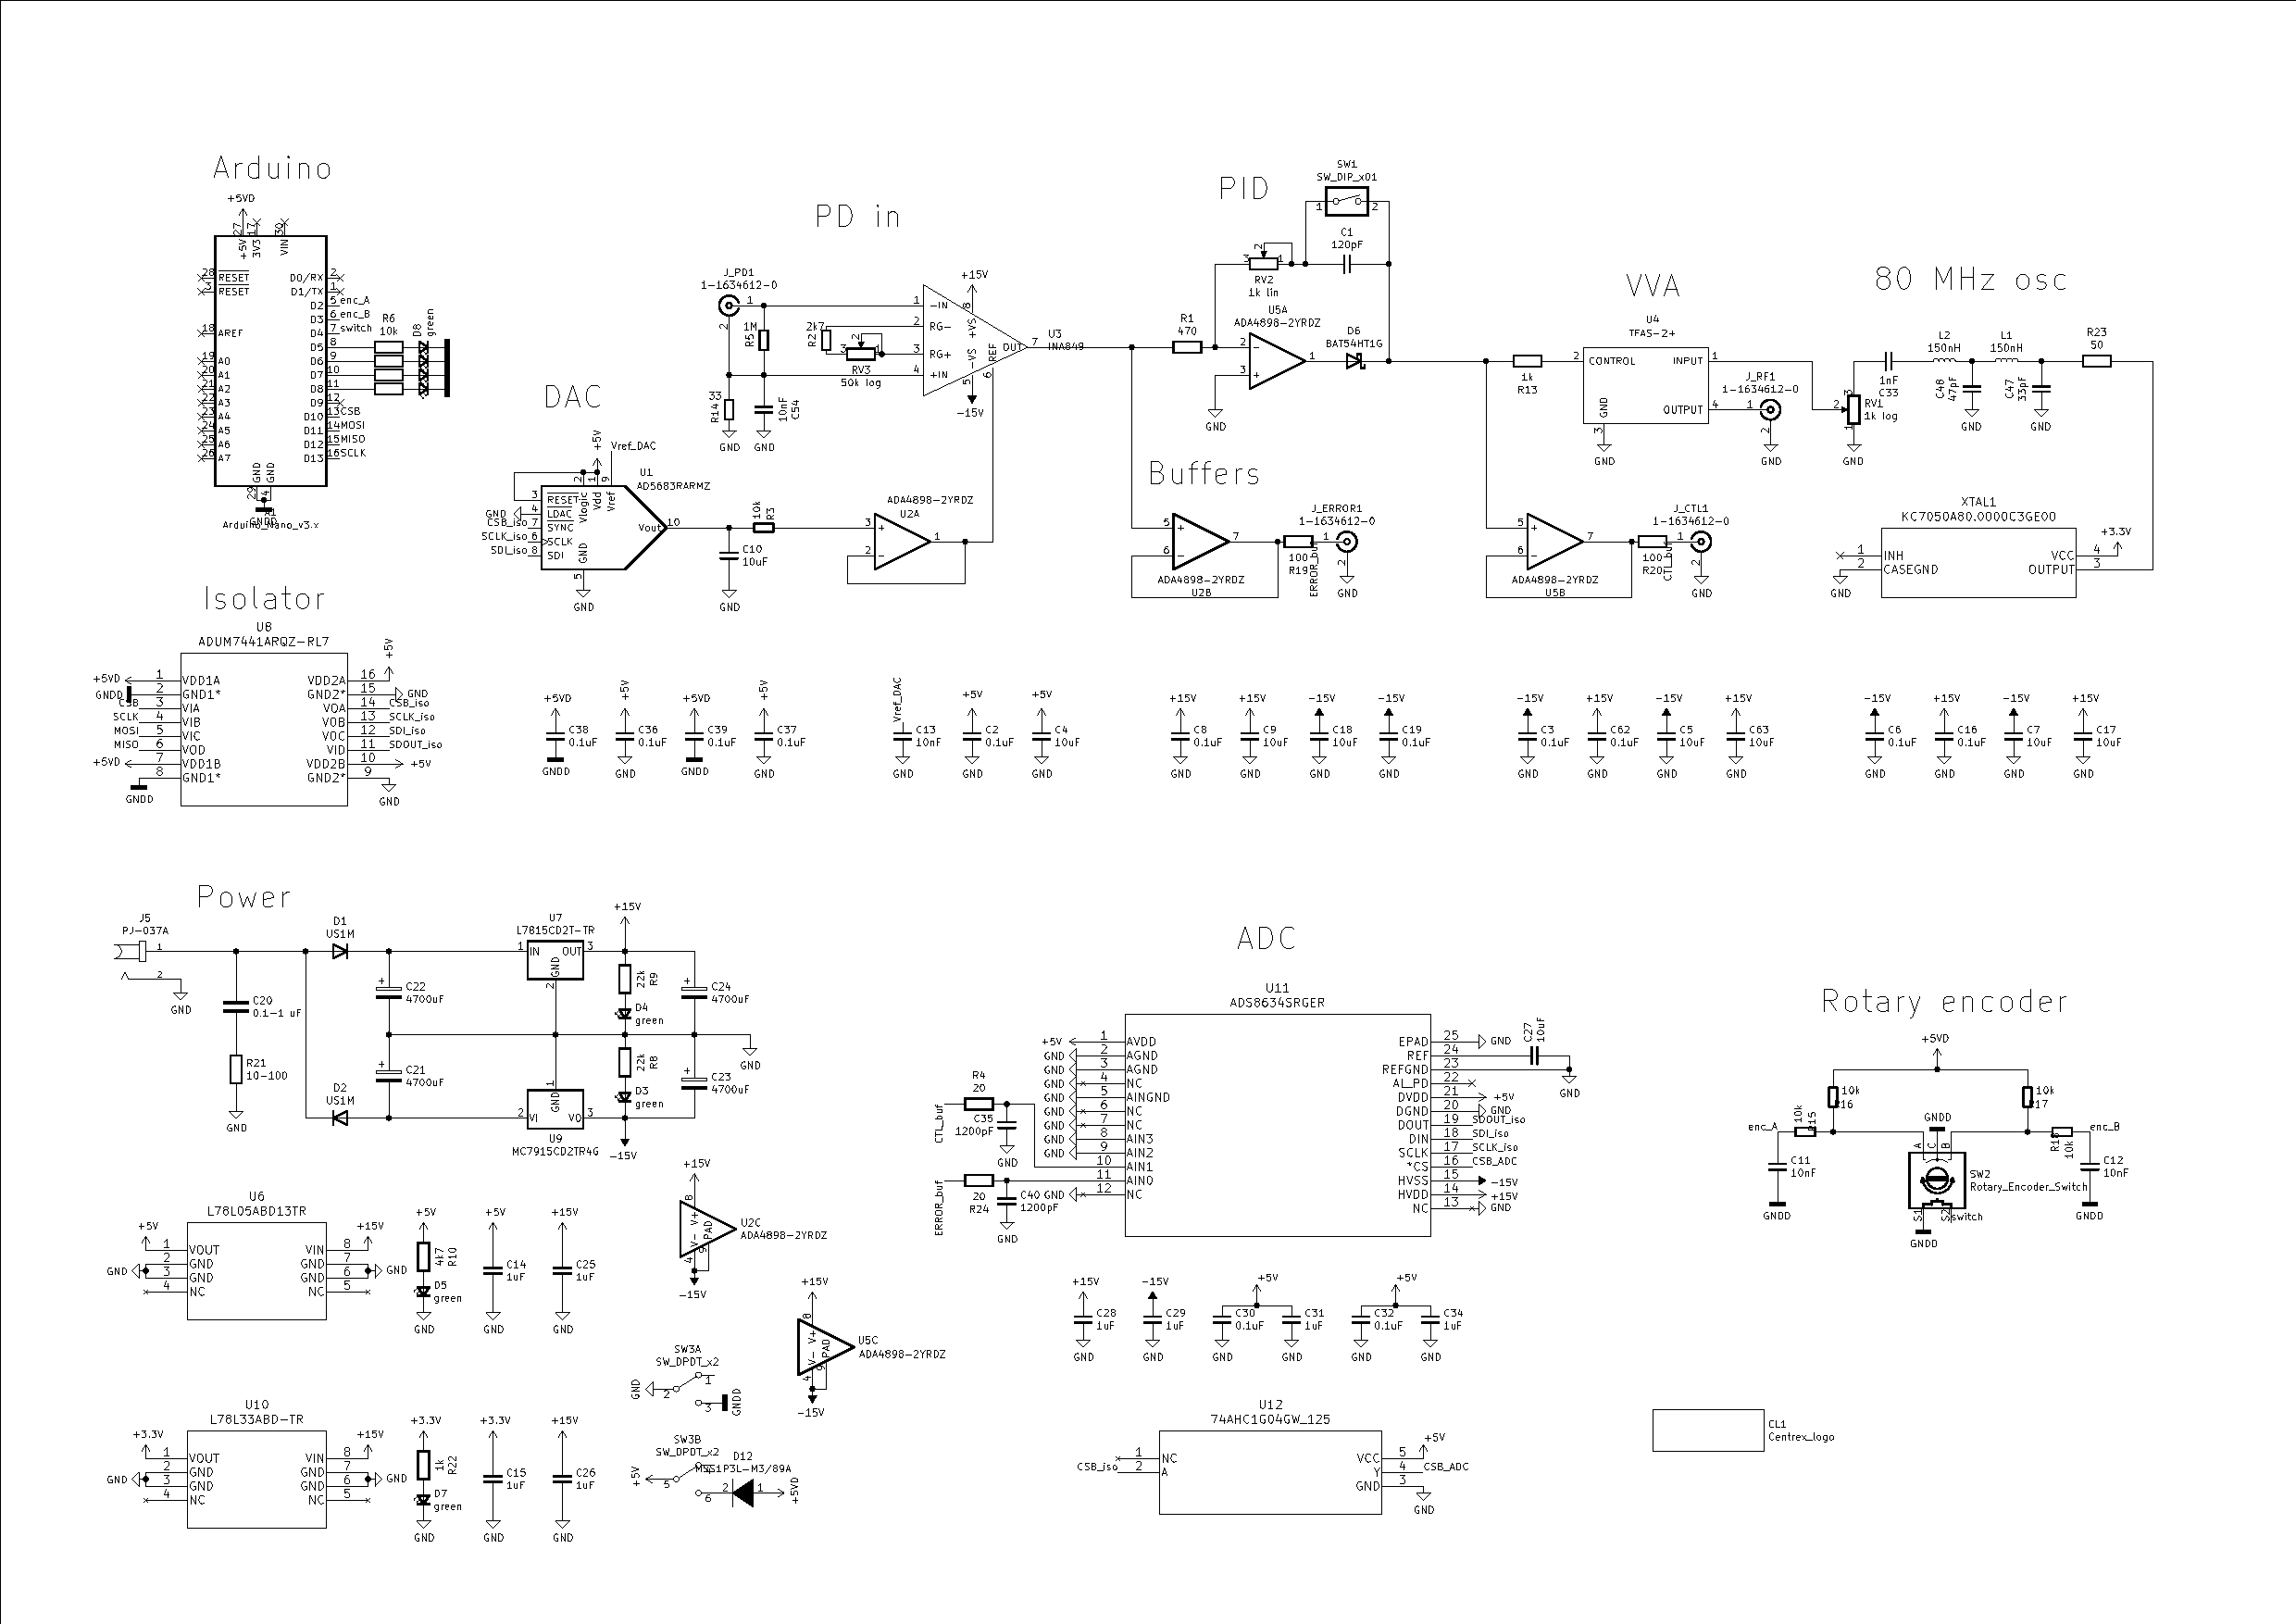
\includegraphics[width=\textwidth]{figs/schematics/laserPIDpower.pdf}
   \caption{LaserPIDpower v2.3 schematic.}
  \label{laserPIDpower_schem}
\end{figure}

The control loop consists of a simple integrator (U5A, ADA4898-2YRDZ). (While we
call this a PID controller, in practice we only use the `I' part.) The
integrator has an adjustable time constant via the potentiometer RV2 (1k lin)
and the fixed capacitor C1 (120pF). In order to disable integral control, the
capacitor can be shorted out by a DIP switch SW1. Furthermore, only the positive
polarity of the control output makes sense (the RF output can be at full power
or attenuated, but not `negative' since it is an AC signal). The diode D6
(BAT54HT1G) ensures that there is only one polarity of the control output (to
within a diode drop, approx.\ 0.2~V for the Schottky diode). A buffered control
output is available from the BNC connector J\_CTL1.

The control voltage is then used to modulate the amplitude of an RF signal. The
modulation is done using a bi-phase pin diode switch (TFAS-2+) used as a
voltage-varying attenuator (VVA). The RF signal itself is generated using an
80~MHz crystal oscillator (KC7050A80.0000C3GE00) filtered through a fourth-order
low-pass filter (L1=150nH, C47=33pF, L2=150nH, C48=47pF) and optionally
attenuated by a potentiometer (RV1, 1k log). The RF output is available from
the BNC connector J\_RF1.

To facilitate the use of the board without access to a computer, the
microcontroller also reads a rotary encoder to set the setpoint. Pressing down
on the encoder switches between different levels of coarseness of adjustment.

\begin{figure}
   \centering
  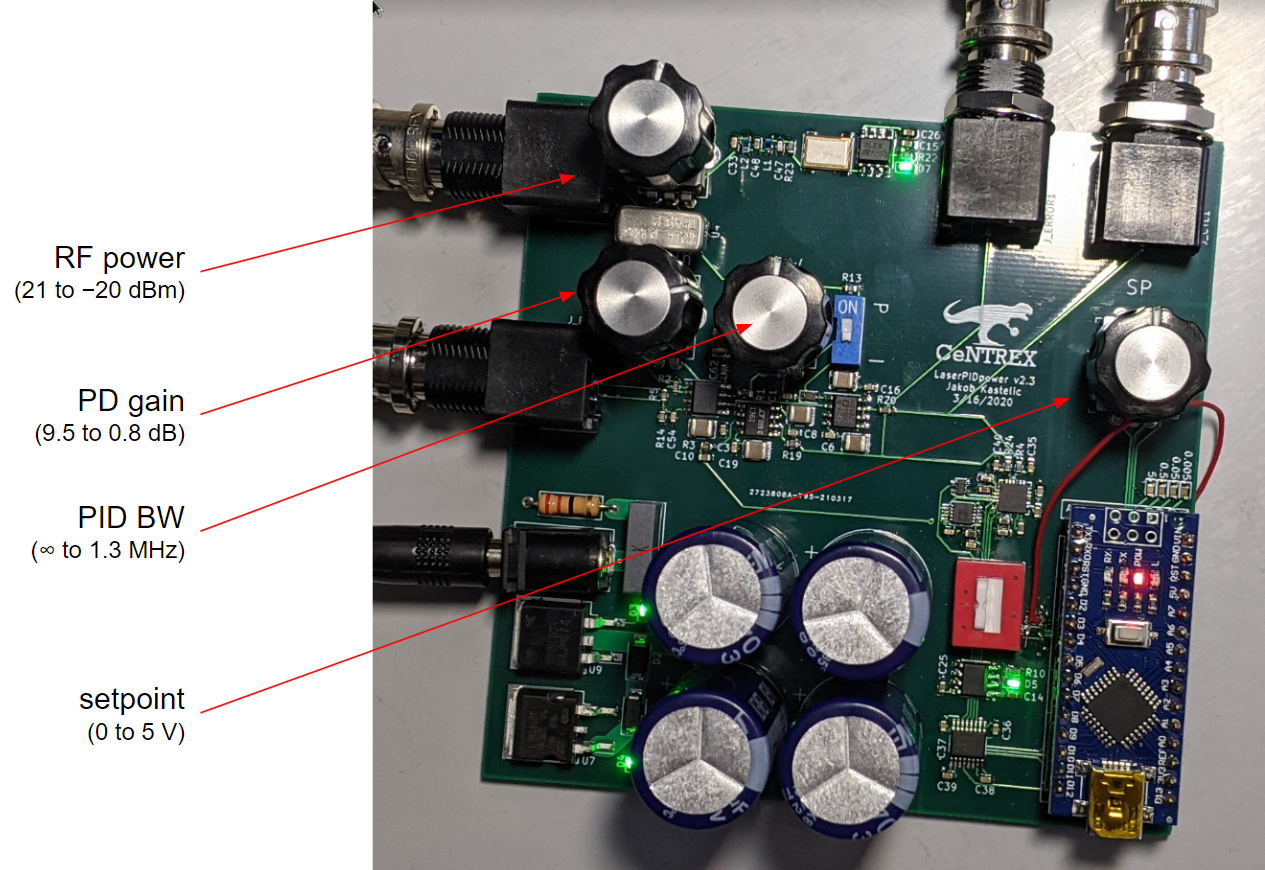
\includegraphics[width=.49\textwidth]{figs/todo/laserPIDpower.png}
  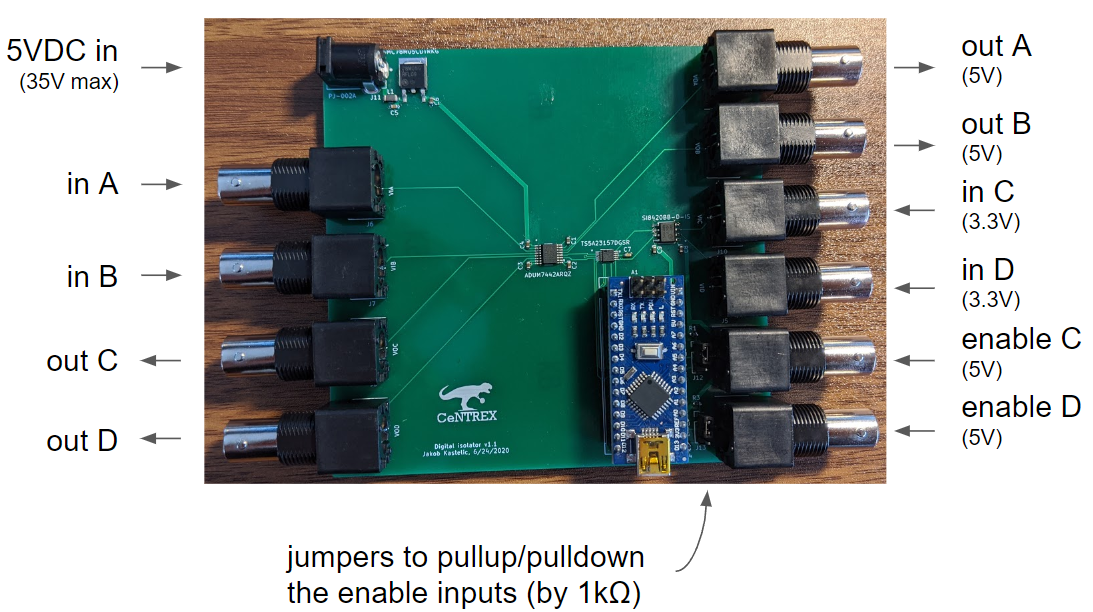
\includegraphics[width=.49\textwidth]{figs/todo/isolator.png}
   \caption[LaserPIDpower v2.3, Digital isolator v1.1.]{\part{Left}
   LaserPIDpower v2.3. Connections, clockwise from top right: control out, error
   out, RF out, PD in, 16VAC in. \part{Right} Digital
   isolator v1.1.}
  \label{laser_PCB}
\end{figure}

\subsection{Digital isolator for laser}

The Digital isolator circuit (schematic in Fig.~\ref{digitalIsolator_schem}, PCB
in Fig.~\ref{laser_PCB}) provides high-voltage isolation for four signal lines,
two per direction. We use this circuit to protect the Programmable TTL Pulse
Generator (PulseBlaster) from damaging transients generated by the YAG laser
control electronics. Furthermore, two of the control lines (C and D) can be
gated by a computer through the Arduino or TTL signals via the provided BNC
ports. The circuit is powered directly by 5V DC and not an AC voltage like most
of the other circuits.

\subsection{Shim coils: current source, relays}

\paragraph{Current source}

The Shim coils circuit (schematic in Fig.~\ref{shimcoils_schem}, PCB
in Fig.~\ref{coils_PCB}) is a 16-channel bipolar approx.\ $\pm10$~mA current
source used to control the shim coils in the magnetic field control system.
Since there are five sets of 16 coils, we use five copies of this PCB connected
to a USB hub in order to control all the coils from a computer.

\begin{figure}
   \centering
  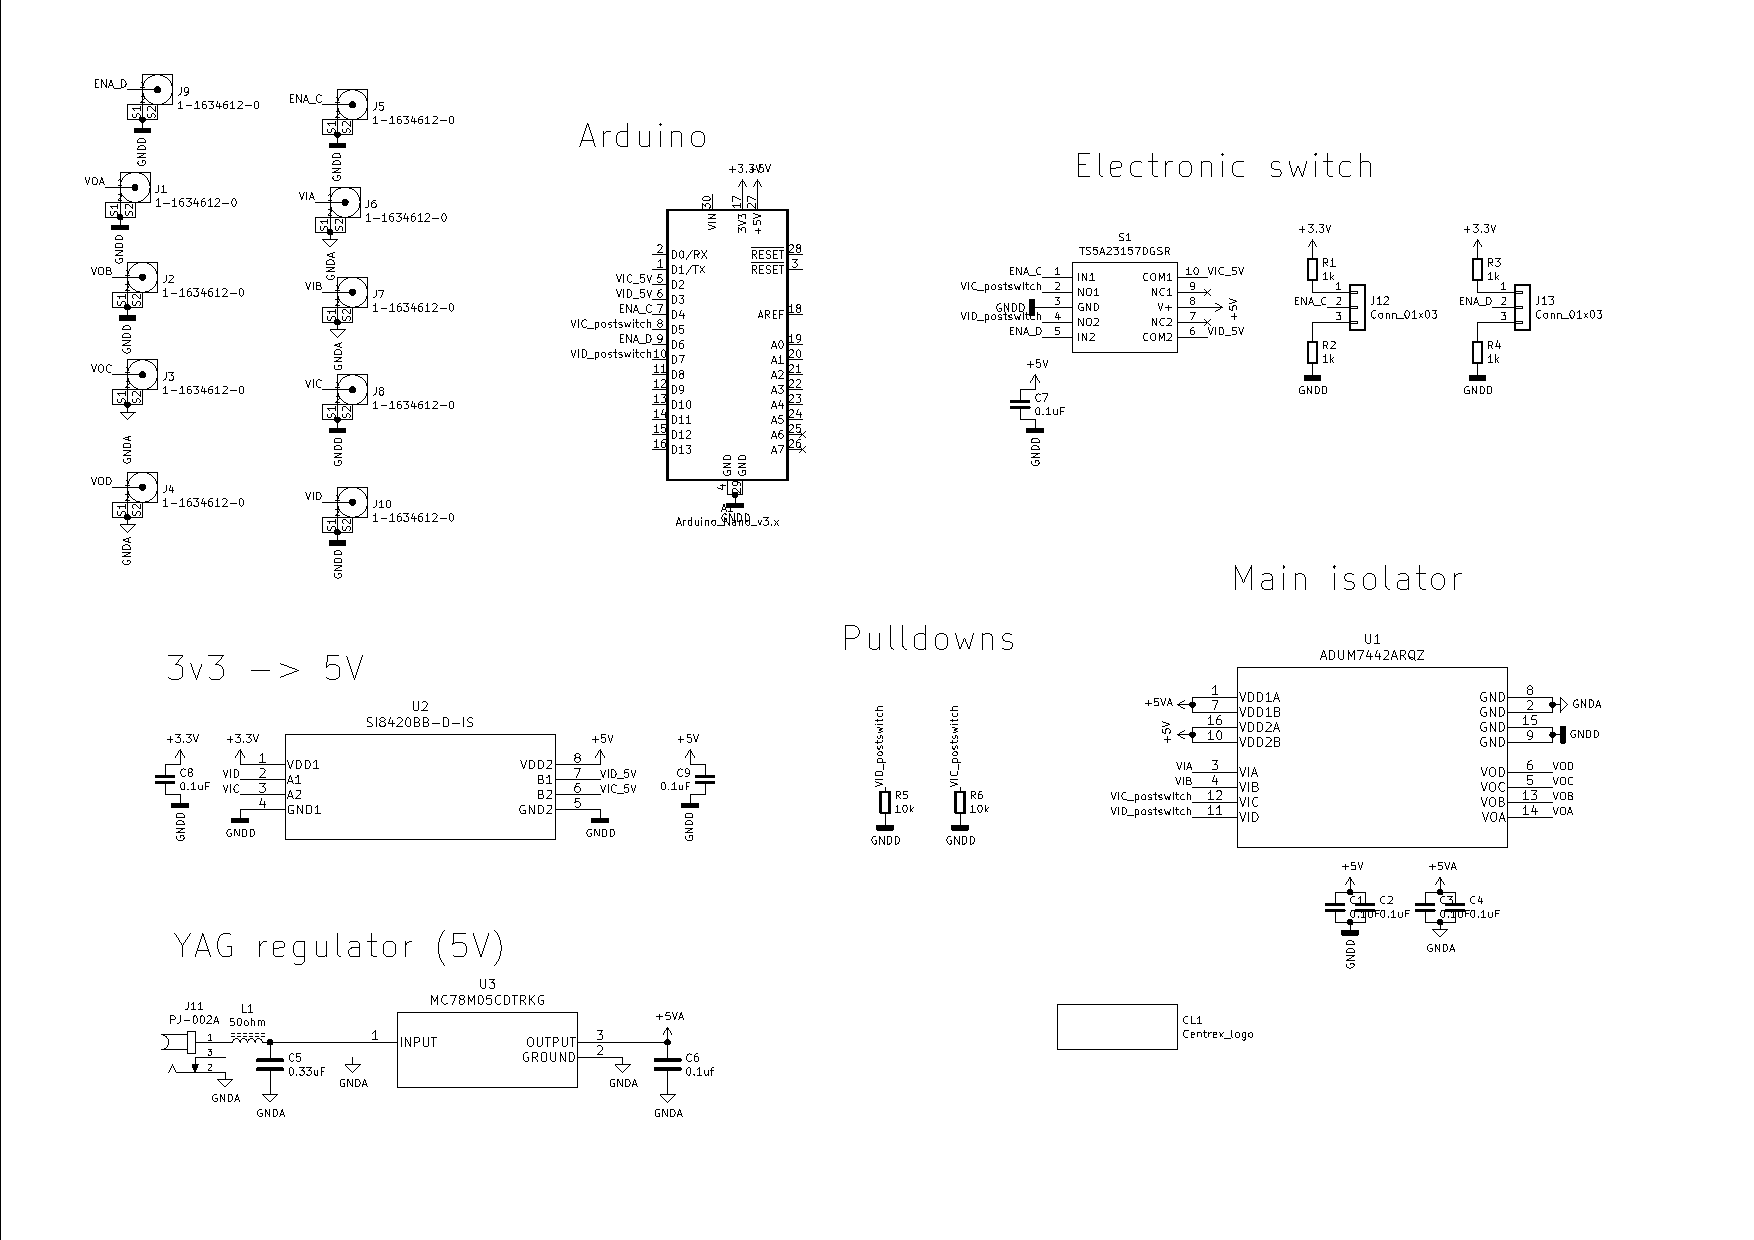
\includegraphics[width=\textwidth]{figs/schematics/digitalIsolator.pdf}
   \caption{Digital isolator v1.1 schematic.}
  \label{digitalIsolator_schem}
\end{figure}

The circuit uses an Arduino to control two 8-channel voltage-output DACs (U1 and
U37, AD5676RBRUZ) via a digital isolator (U4, ADUM7441ARQZ-RL7). Originally,
this circuit used a single 16-channel DAC, which became hard to obtain due to
the global chip shortage. I have thus adapted the board to the two 8-channel
DACs, and in order to avoid having to change the digital isolator to add another
CS line, I generate it using an inverter (U38, SN74LVC1GU04DRLR).

The current source section of the circuit is identical between the 16 outputs
and consists of a unity-gain differential amplifier (AD8276) and an opamp
follower (OP07). The differential amplifier outputs the difference between a DAC
voltage and a mid-scale reference voltage, thus generating a bipolar voltage
from a unipolar DAC output. The current from the differential amplifier is
passed through a precision 100~$\Omega$ resistor (RQ73C1J100RBTD, 0.1\%,
10~ppm/\degC), and then into the load, which returns the current to ground. The
opamp follower reads the voltage (with respect to ground) of the resistor
`output' (the part connected to the load) and feeds it into the differential
amplifier's reference input. Thus the differential amplifier strives to set a
constant voltage on one side of the resistor with respect to the other; this
constant voltage drop across a precision resistor is what creates a constant
current output. This circuit is also shown in
\cite[Fig.~5.69A]{horowitz2016art}.

\begin{figure}
   \centering
  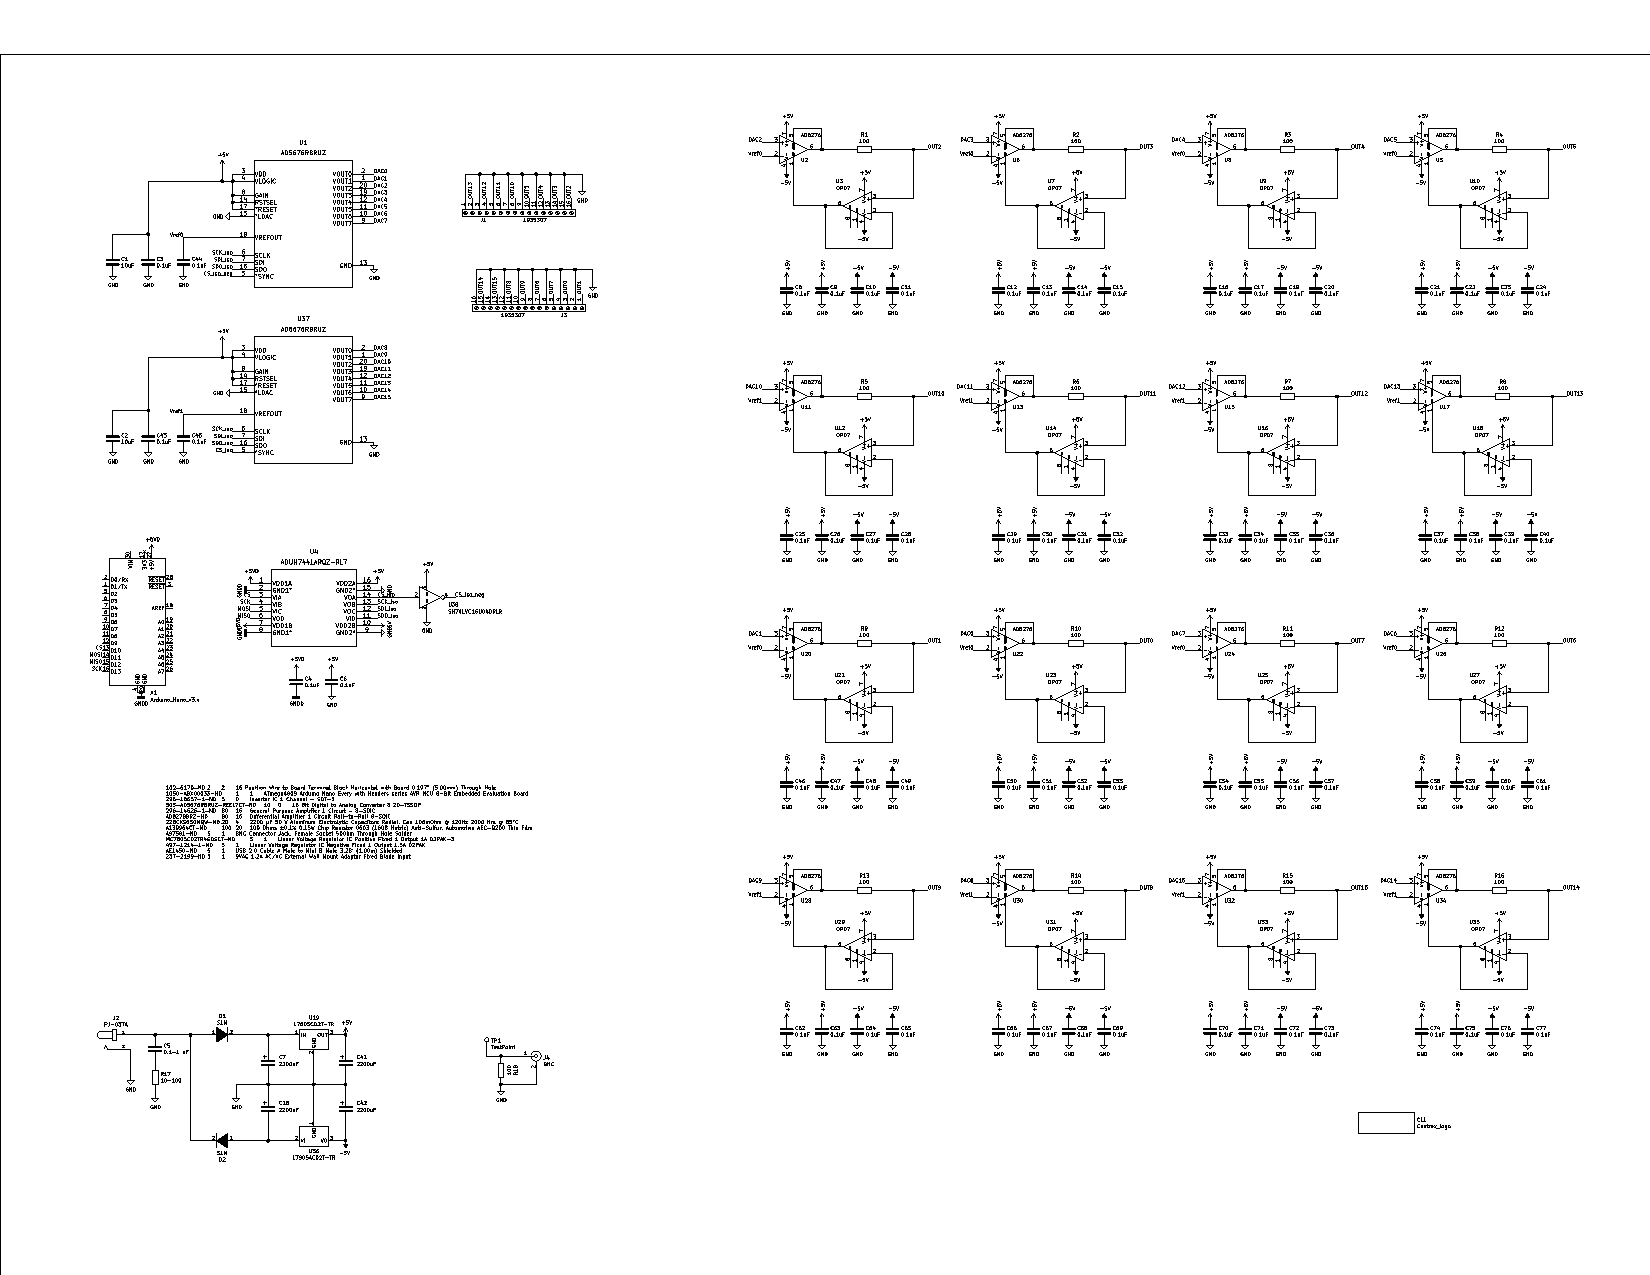
\includegraphics[width=\textwidth]{figs/schematics/shimcoils.pdf}
   \caption{Shim coils v1.3a schematic.}
  \label{shimcoils_schem}
\end{figure}

The power section is as described at the top of this chapter. A low-voltage AC
input is rectified by two diodes (D1, D2, type S1M) of opposite orientations to
provide the positive and negative voltages, which are then regulated (U19,
L7805CD2T-TR, U36, L7905ACD2T-TR). The series $RC$ connected across the
transformer secondary right where the low-voltage AC reaches the PCB (C5, R17)
suppressed a train of periodic sharp spikes of relatively large amplitude that
can sometimes occur with certain transformers. \cite[sect~9.5.3C]{horowitz2016art}

\paragraph{Relay board}

The Shim\_relays circuit (schematic in Fig.~\ref{shimrelays_schem}, PCB
in Fig.~\ref{coils_PCB}) is placed between the shim coils and the current source
described above in order to be able to disconnect all shim coils for testing and
calibration purposes using a computer command. Each coil is connected using a
relay which can be individually controlled, enabling the control over each
coil separately. The circuit is very simple and merely provides a connection
between the microcontroller (Arduino) and the relays (AZ822-2C-12DE) via digital
isolators (ADUM3400CRWZ-RL).

\begin{figure}
   \centering
  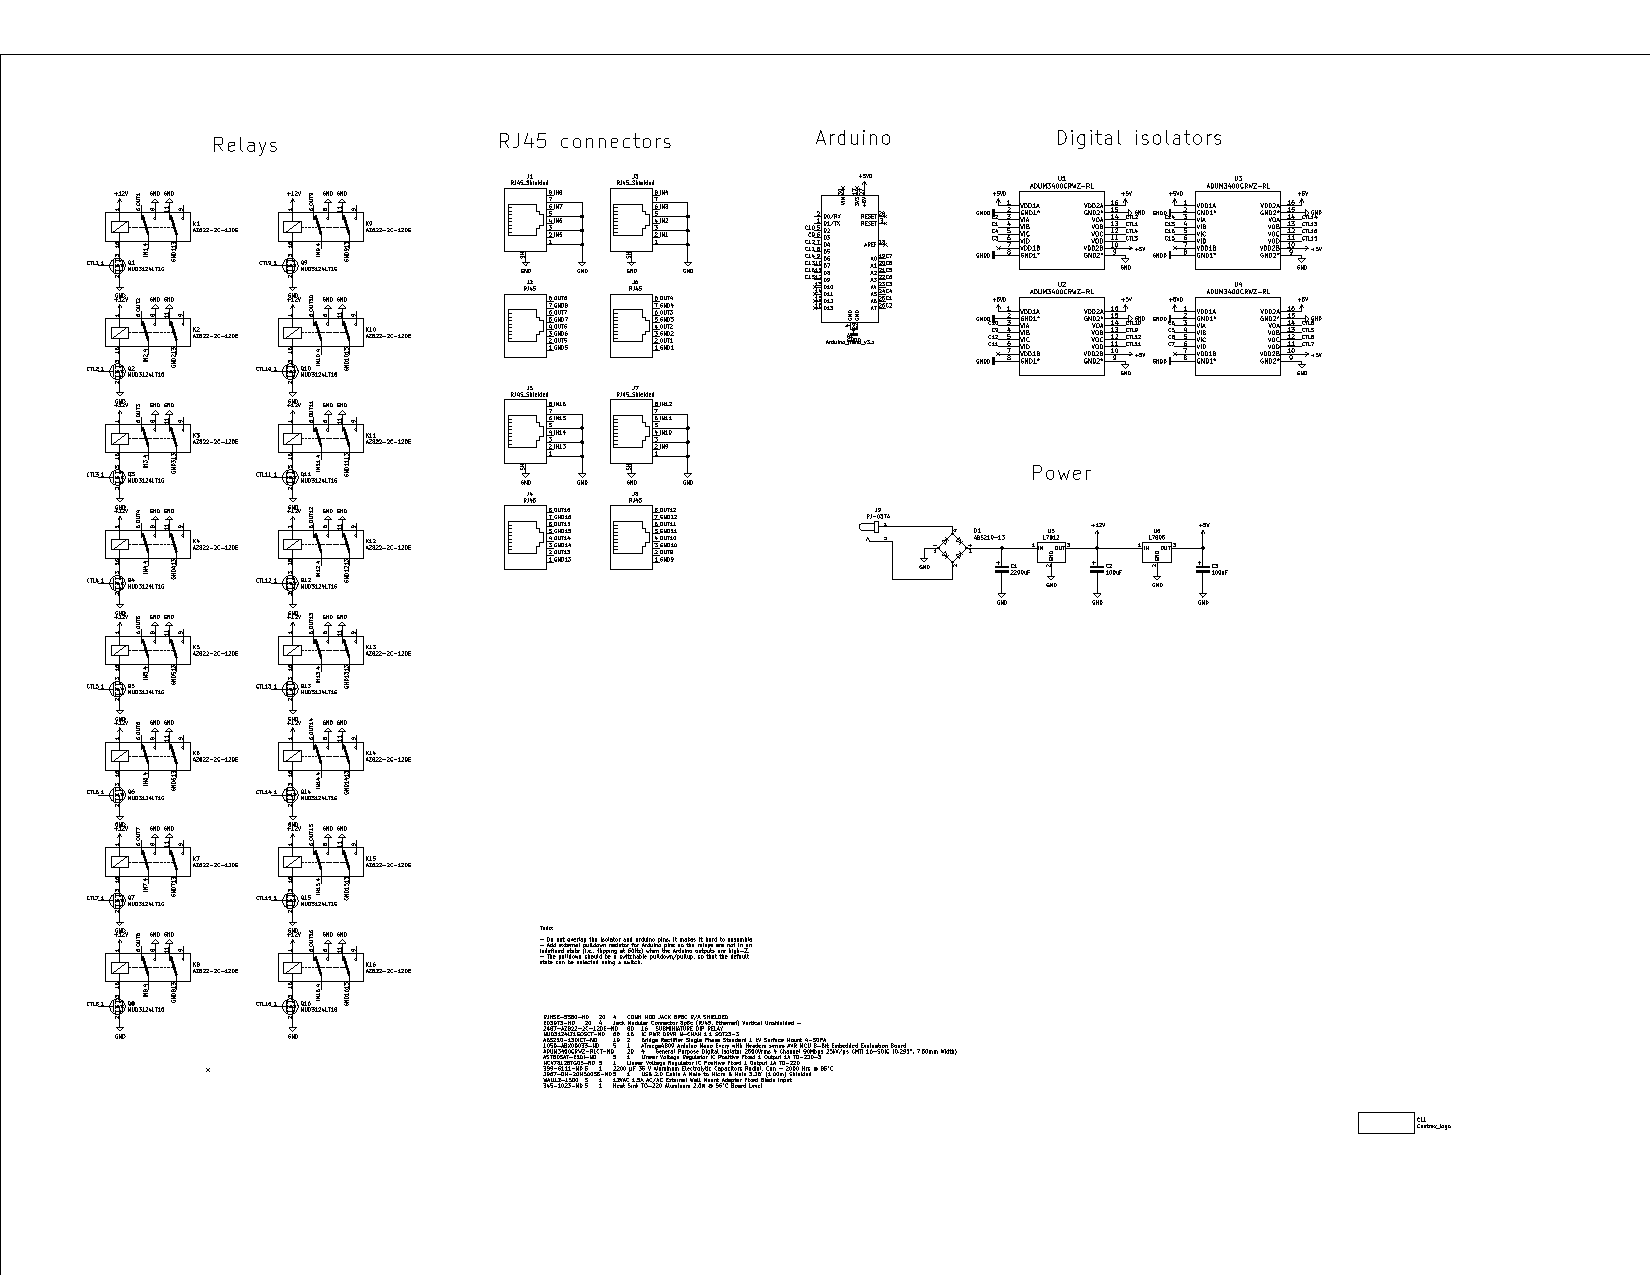
\includegraphics[width=\textwidth]{figs/schematics/shimrelays.pdf}
   \caption{Shim\_relays v1.0 schematic.}
  \label{shimrelays_schem}
\end{figure}

\begin{figure}
   \centering
  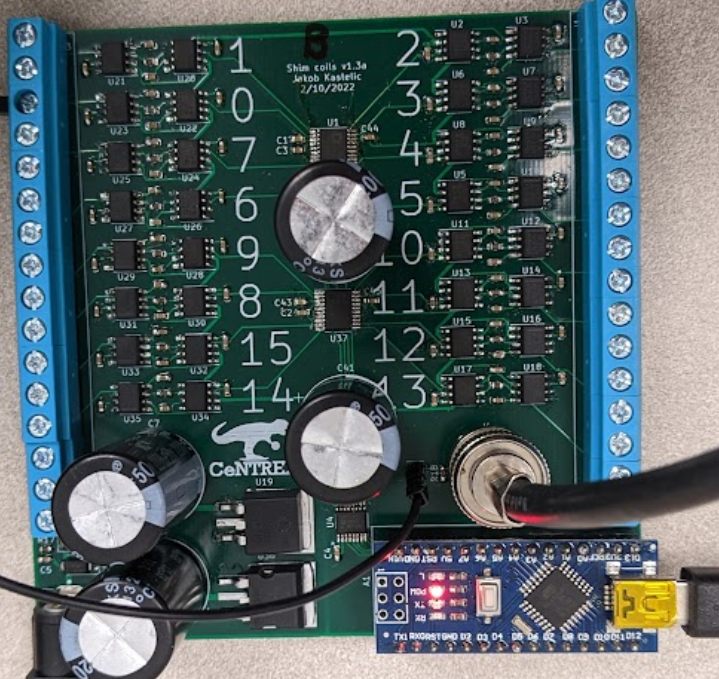
\includegraphics[width=.49\textwidth]{figs/todo/coils.png}
  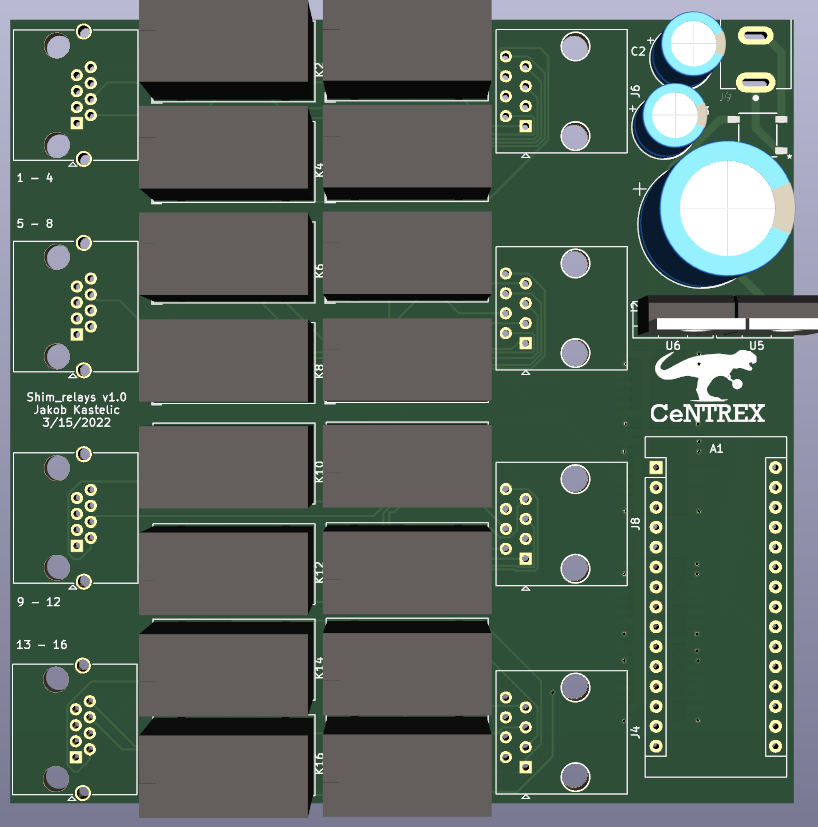
\includegraphics[width=.49\textwidth]{figs/todo/shimrelays.png}
   \caption[Shim coils v1.3a, Shim\_relays v1.0.]{\part{Left} Shim coils v1.3a.
   \part{Right} Shim\_relays v1.0.  Connections, counter-clockwise from bottom
   left: in 13--16, in 9--12, in 5--8, in 1--4, out 1--4, in 12VAC, out 5--8,
   out 9--12, out 13--16. Since the PCBs are currently in use, only a rendered
   drawing is shown here, which does not show the RJ45 (`ethernet') connectors
   nor the Arduino Nano board (lower right, under the \CENTREX\ logo).}
  \label{coils_PCB}
\end{figure}


\subsection{Degaussing: DAC, relays}

\paragraph{Relay board}

The Degaussing relay board circuit (schematic in
Fig.~\ref{degaussingrelay_schem}, PCB in Fig.~\ref{deg_PCB}) is used to
connect the degaussing coils to a decaying sinusoidal degaussing signal. The
coils are always only connected one at a time, starting from the degaussing coil
of the outermost shield layer, and ending with the innermost coil. While the
magnetic shield only consists of four layers, the PCB has a fifth connection
available for redundancy.

The decaying sinusoidal signal is generated by the DAC board (described below),
amplified by a power amplifier (Kepco BOP36-12M), passed through an isolation
transformer (Hammond 169J) to remove the DC offset, and input into degaussing
relay board through the screw terminal J1. The current then passes through a
fuse and a 1~$\Omega$ power resistor (with a heat sink), and then via the relays
into individual coils, connected to the screw terminals (J2, J4, J5, J6, J7).

There are two opamp followers that provide a buffered copy of the voltage (with
respect to the ground) of the two terminals of the high-power resistor. The
difference between these two voltages could in principle be used to monitor the
degaussing current. In practice, the opamps can be damaged when degaussing at a
voltage higher than the $\pm5$~V opamp supply, in which case the current readout
does not work. In the next version of the circuit, the opamps should be powered
from at least a $\pm12$~V supply.

\begin{figure}
   \centering
  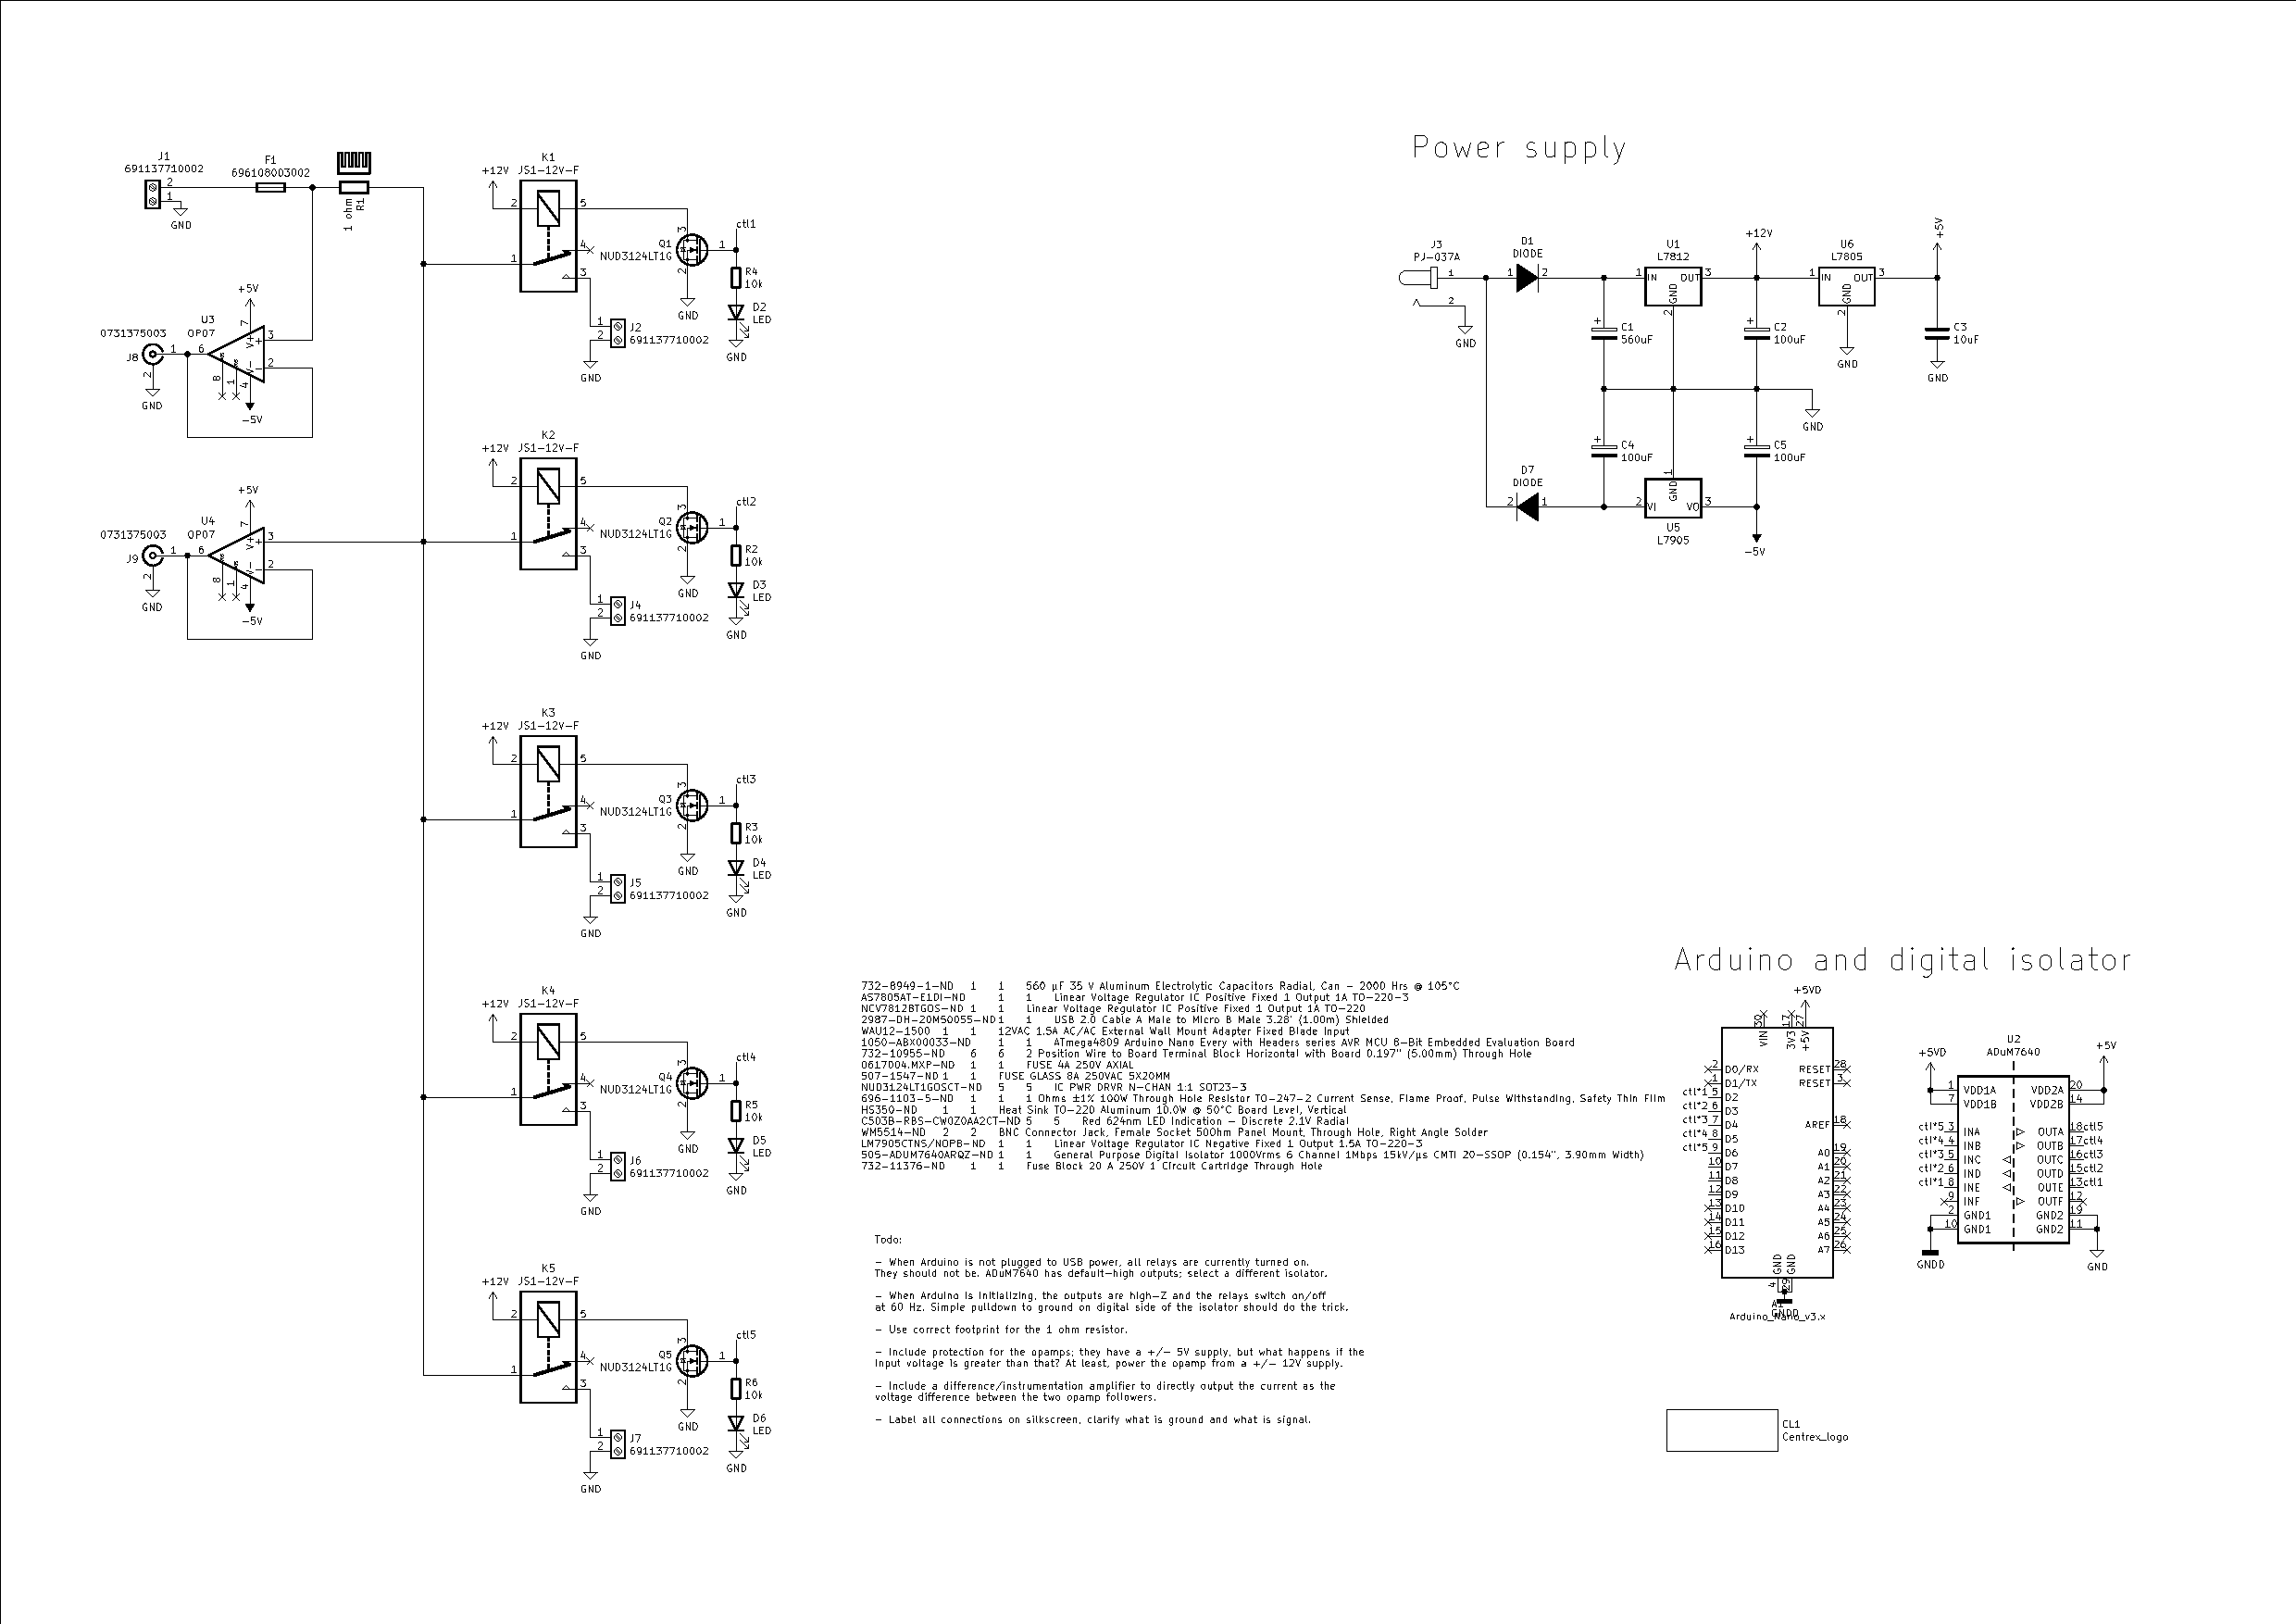
\includegraphics[width=\textwidth]{figs/schematics/degaussingRelay.pdf}
   \caption{Degaussing relay board v1.3 schematic.}
  \label{degaussingrelay_schem}
\end{figure}

\paragraph{DAC board}

The Degaussing DAC board circuit (schematic in Fig.~\ref{degaussingDAC_schem},
PCB in Fig.~\ref{deg_PCB}) is used to generate a decaying sinusoidal signal to
drive the degaussing coils. It consists of a high-speed microcontroller (ARM
Cortex-M7 at 600 MHz on a Teensy 4.0 board) that controls a DAC (AD5761BRUZ) via
a digital isolator (ADUM7441ARQZ-RL7). The DAC output is filtered by a simple
low-pass filter (R6=100, C29=1uF) and buffered by an opamp (AD8675ARZ-REEL7)
before being output through a BNC connector at J1.

The signal is not exactly of the form $Ae^{-t/t_0}\sin(\omega t)$, but rather
consists of sinusoidal pulses, such that each pulse has a smaller amplitude than
the preceding pulse. In the main control loop of the microcontroller, the
following \verb|if| statement waits for the user to set
\verb|step_forward=true|.
%
\begin{lstlisting}[language=C++]
const unsigned int amp_max = 65535
if (step_forward) {
   amp /= div_f;
   for (int i=0; i<amp_max; i+=di) {
      write_SPI( amp_f*amp*sin(2*3.14159*i/amp_max)/2 + amp_max/2 );
      delayMicroseconds(dt);
   }
      step_forward = false;
}
\end{lstlisting}
%
When that happens, the amplitude (initially set to
\verb|amp=amp_max|) is divided down by a factor \verb|div_f|, and a single
sinusoidal pulse is written to the DAC (in units of steps size \verb|di| at time
increments \verb|dt| microseconds) via the SPI line. Finally,
\verb|step_forward| is deactivated, waiting for the next pulse to be requested
by the user.

\begin{figure}
   \centering
  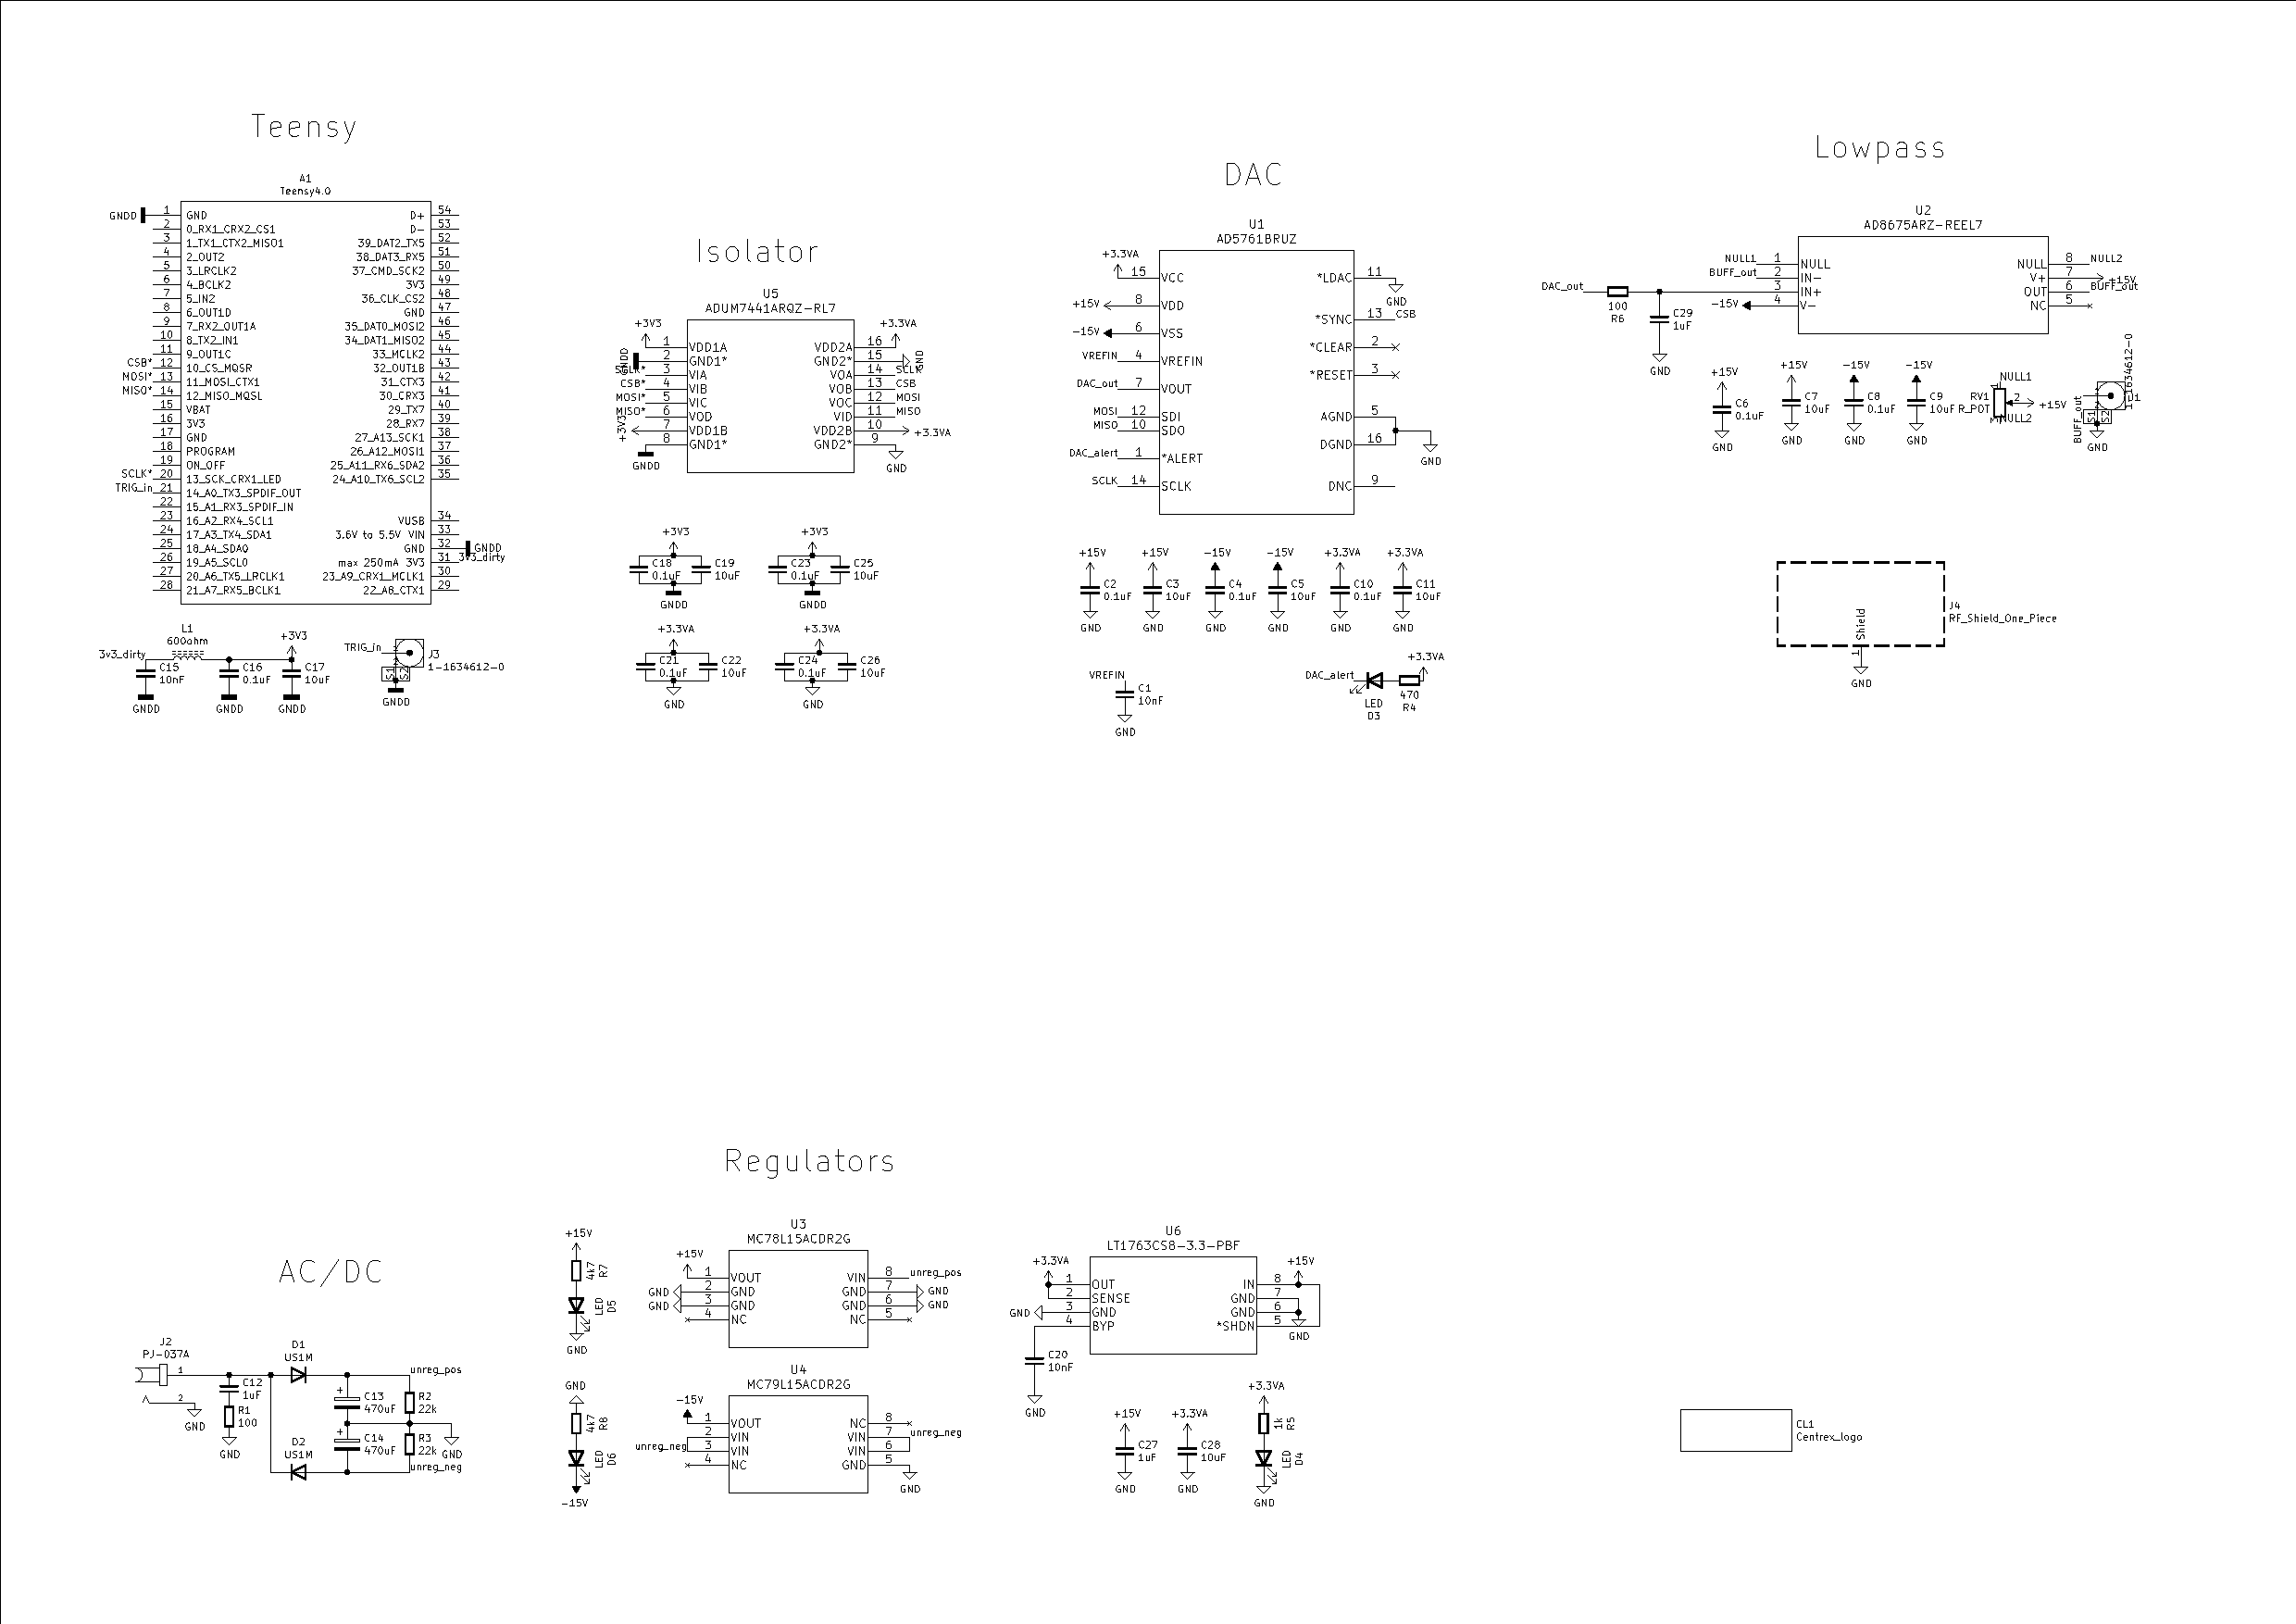
\includegraphics[width=\textwidth]{figs/schematics/degaussingDAC.pdf}
   \caption{Degaussing DAC board v2.0 schematic.}
  \label{degaussingDAC_schem}
\end{figure}

\begin{figure}
   \centering
  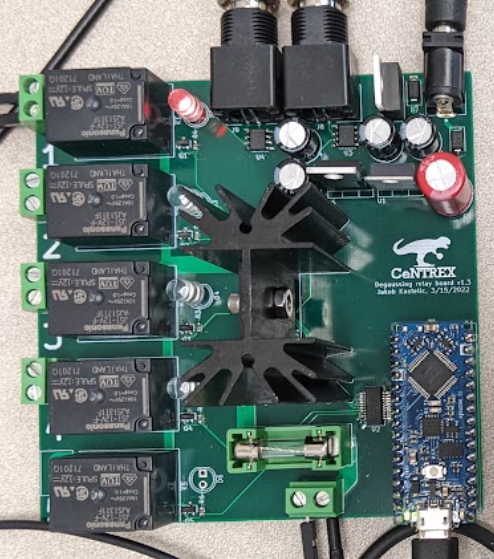
\includegraphics[width=.49\textwidth]{figs/todo/degaussing_relays.png}
  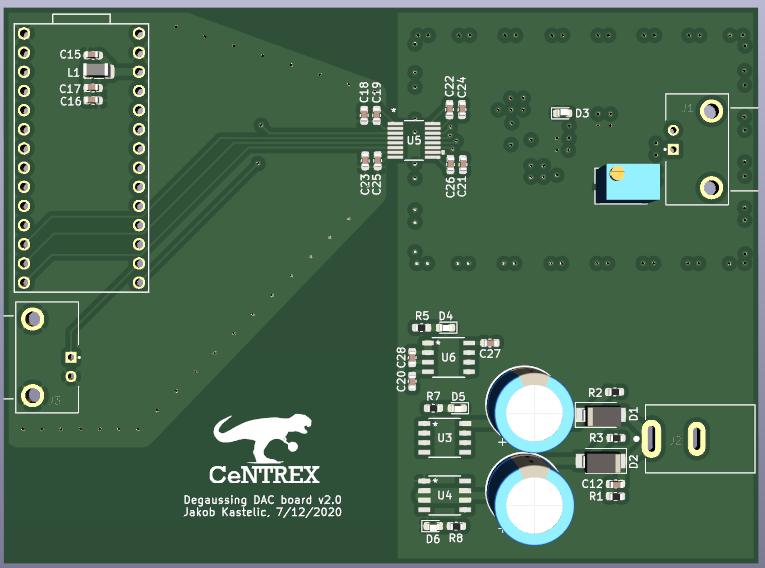
\includegraphics[width=.49\textwidth]{figs/todo/deg_DAC.png}
   \caption[Degaussing relay board v1.3, Degaussing DAC board v2.0.]{\part{Left}
   Degaussing relay board v1.3. Connections, clockwise from top right: in 12VAC,
   buffered out J8, buffered out J9, coil 1, coil 2, coil 3, coil 4, coil 5, AC
   in (from isolation transformer).\part{Right} Degaussing DAC board v2.0.
   Connections on the right: BNC for DAC output, 16VAC in.}
  \label{deg_PCB}
\end{figure}


\subsection{DecaPSU: ADC board, preamp board}

The precision magnetometers (Bartington Mag-03) are read out in one of two ways.
If only a single sensor is needed, such as when scanning the magnetic field
along the central axis inside the magnetic shield, then the sensor can be
connected to the Bartington SCU-1 unit, which has an adjustable gain for each of
the three axes, as well as selectable low- and high-pass filters. The
conditioned outputs are available from the back of the unit and can be connected
to the ADC board, described in the following, via a custom BNC-to-DB adapter.

Alternatively, if more than one sensor is used, these can be powered by the
Bartington DecaPSU, which outputs the unamplified (but buffered and filtered)
sensor outputs for up two ten 3-axis sensors. The DB output from the DecaPSU can
be directly connected to the ADC board, or can be first amplified using the
preamp board.

\paragraph{ADC board}

The ADC board circuit (schematic in Fig.~\ref{decapsuADC_schem},
PCB in Fig.~\ref{deca_PCB}) is used to digitize up to five 3-axis sensor
outputs. The sensor outputs are directly connected to the inputs of a 16-channel
24-bit DAC (AD4115BCPZ) with $\pm10$~V inputs, with an integrated 5~ppm/\degC\
reference, running from a single 5~V supply. The digital output is read by a
microcontroller board (Teensy 4.0) via a digital isolator (ADUM7441ARQZ-RL7).
The board is powered by a low-voltage AC input voltage, rectified by a diode
bridge (ABS210-13) and regulated (MC78L05ACDR2G).

\begin{figure}
   \centering
  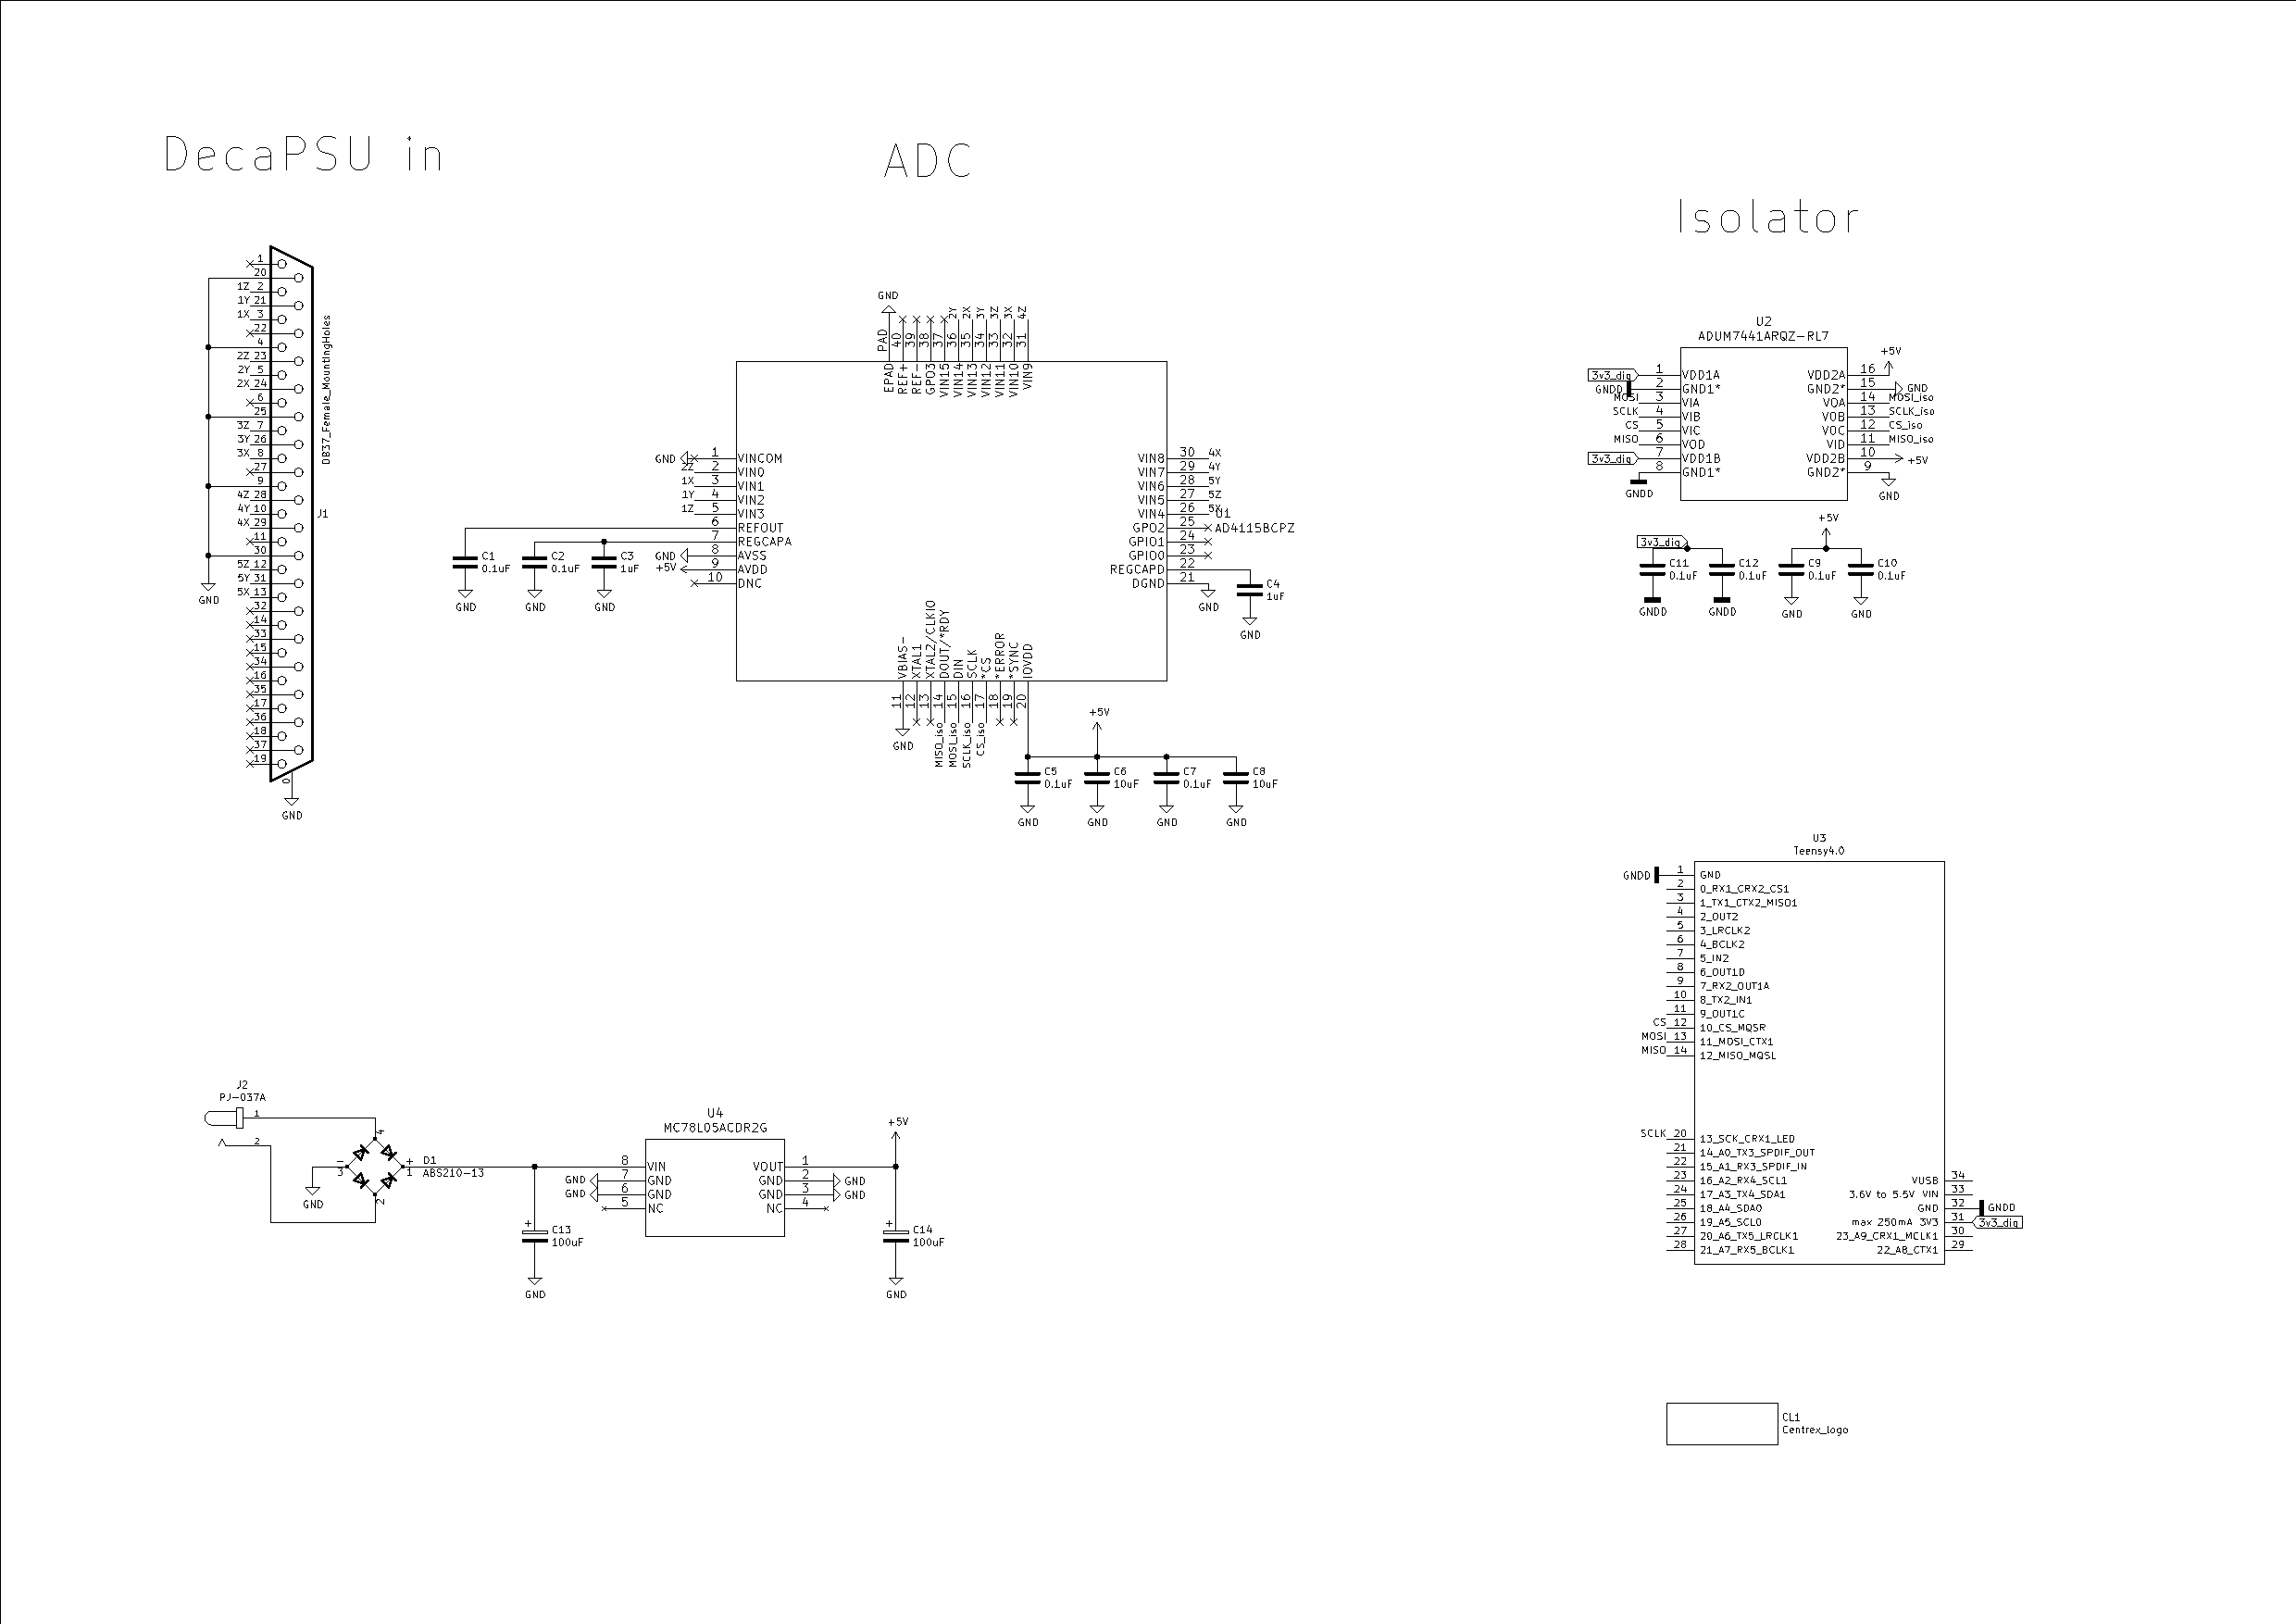
\includegraphics[width=\textwidth]{figs/schematics/decapsuADC.pdf}
   \caption{DecaPSU to ADC v2.0 schematic}
  \label{decapsuADC_schem}
\end{figure}

\begin{figure}
   \centering
  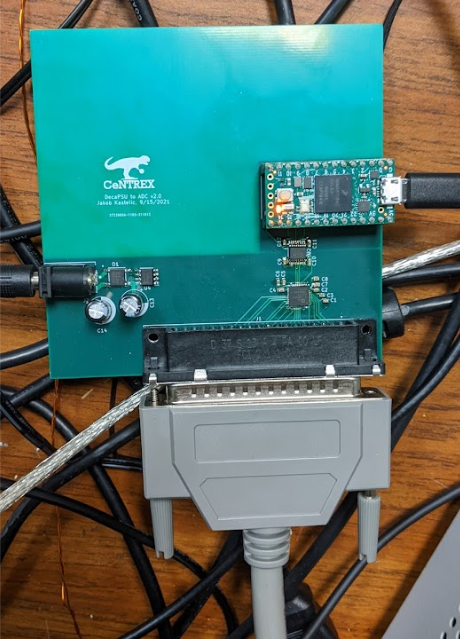
\includegraphics[width=.37\textwidth]{figs/todo/deca_ADC.png}
  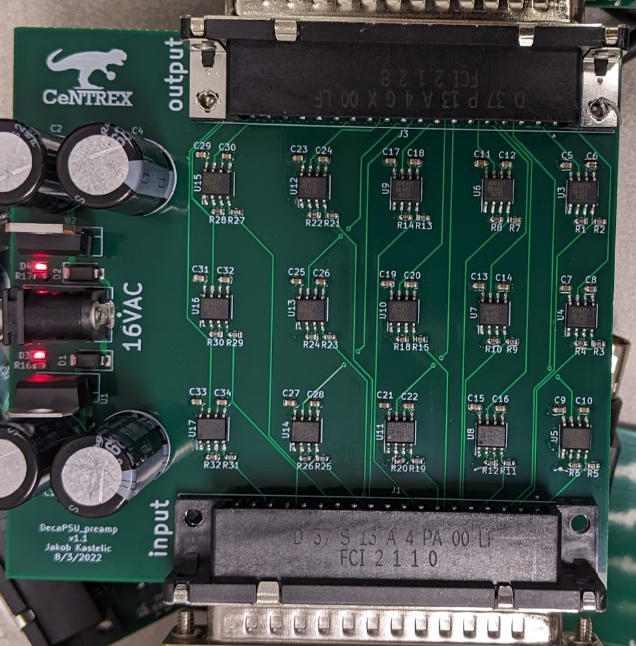
\includegraphics[width=.49\textwidth]{figs/todo/deca_preamp.png}
   \caption[DecaPSU to ADC v2.0, DecaPSU\_preamp v1.1]{\part{Left} DecaPSU to
   ADC v2.0. \part{Right} DecaPSU\_preamp v1.1}
  \label{deca_PCB}
\end{figure}

\paragraph{Preamp board}

The preamp board circuit (schematic in Fig.~\ref{decapsuPreamp_schem},
PCB in Fig.~\ref{deca_PCB}) can be used between the DecaPSU unit and the ADC
board to provide a constant gain of approx.\ 1000 to the sensor signals. It
consists of 15 identical instrumentation amplifier circuits with a precision
$49.9~\Omega$ resistors setting the gain of the amplifier. The board is powered
by a bipolar power supply using two diodes and two linear regulators, very
similar to one described in a previous circuit.

\begin{figure}
   \centering
  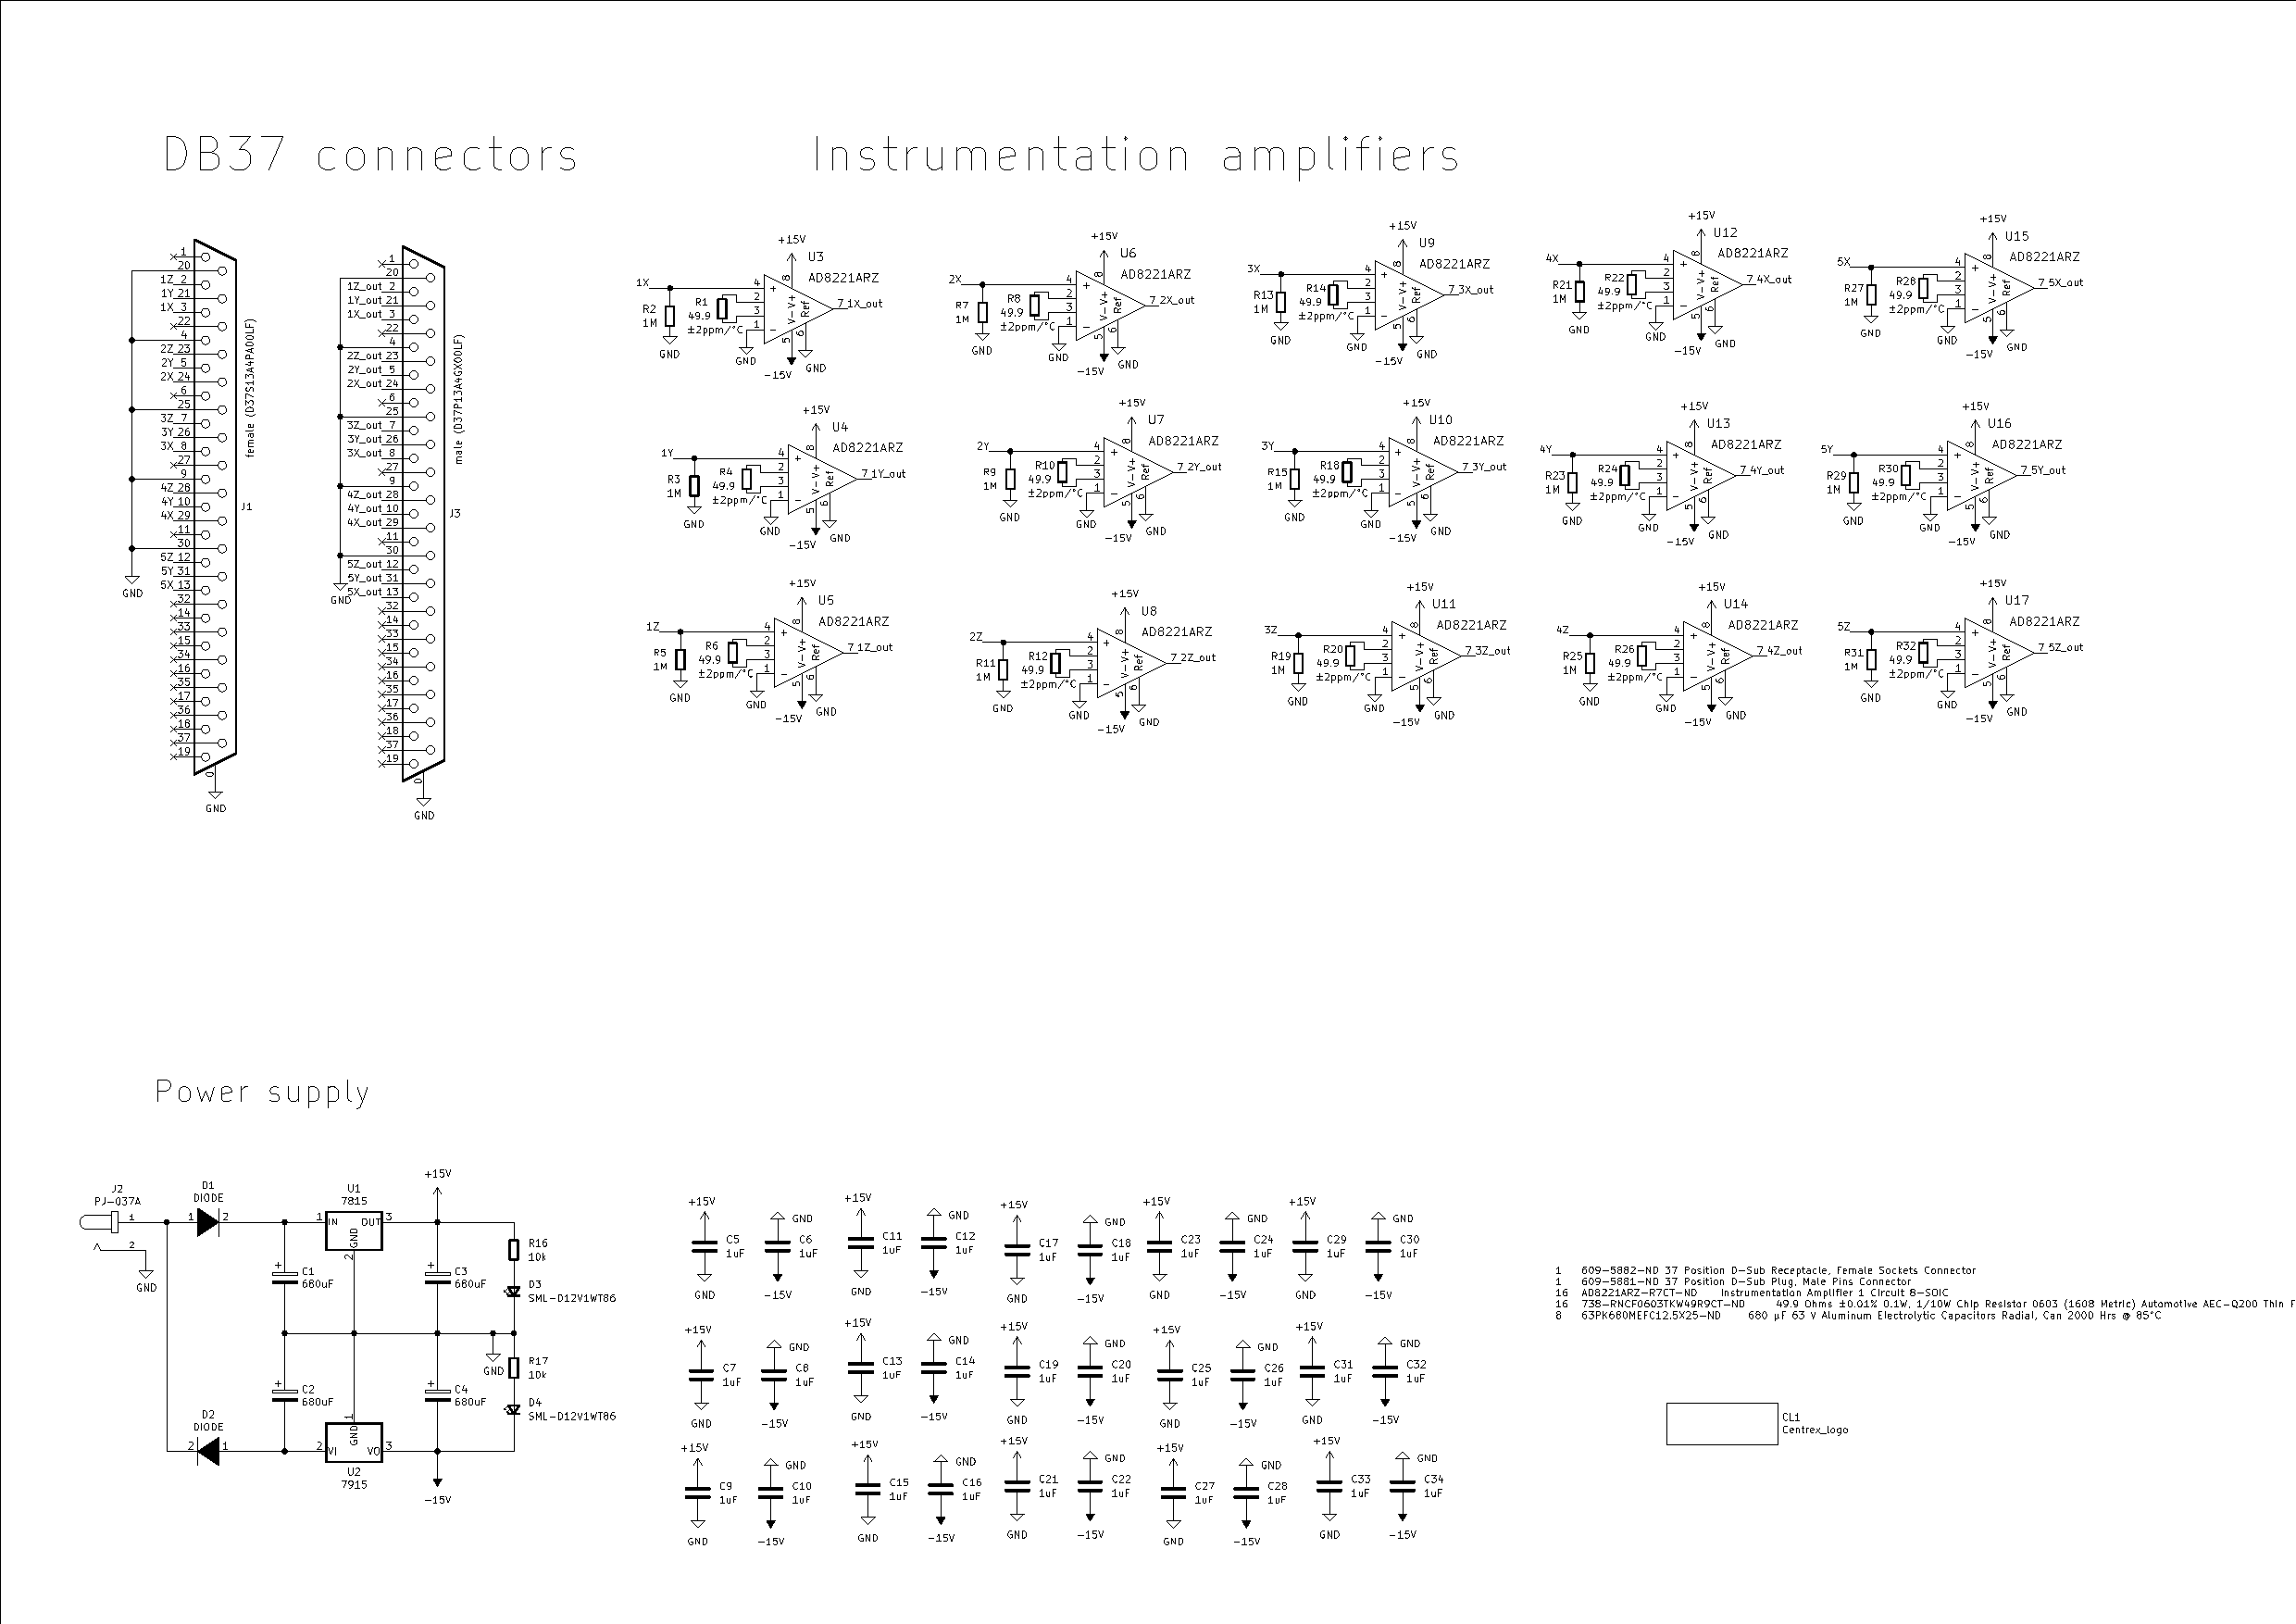
\includegraphics[width=\textwidth]{figs/schematics/decapsuPreamp.pdf}
   \caption{DecaPSU\_preamp v1.1 schematic}
  \label{decapsuPreamp_schem}
\end{figure}


\subsection{Multi ADC and fluxgate magnetometers}

\begin{figure}
   \centering
  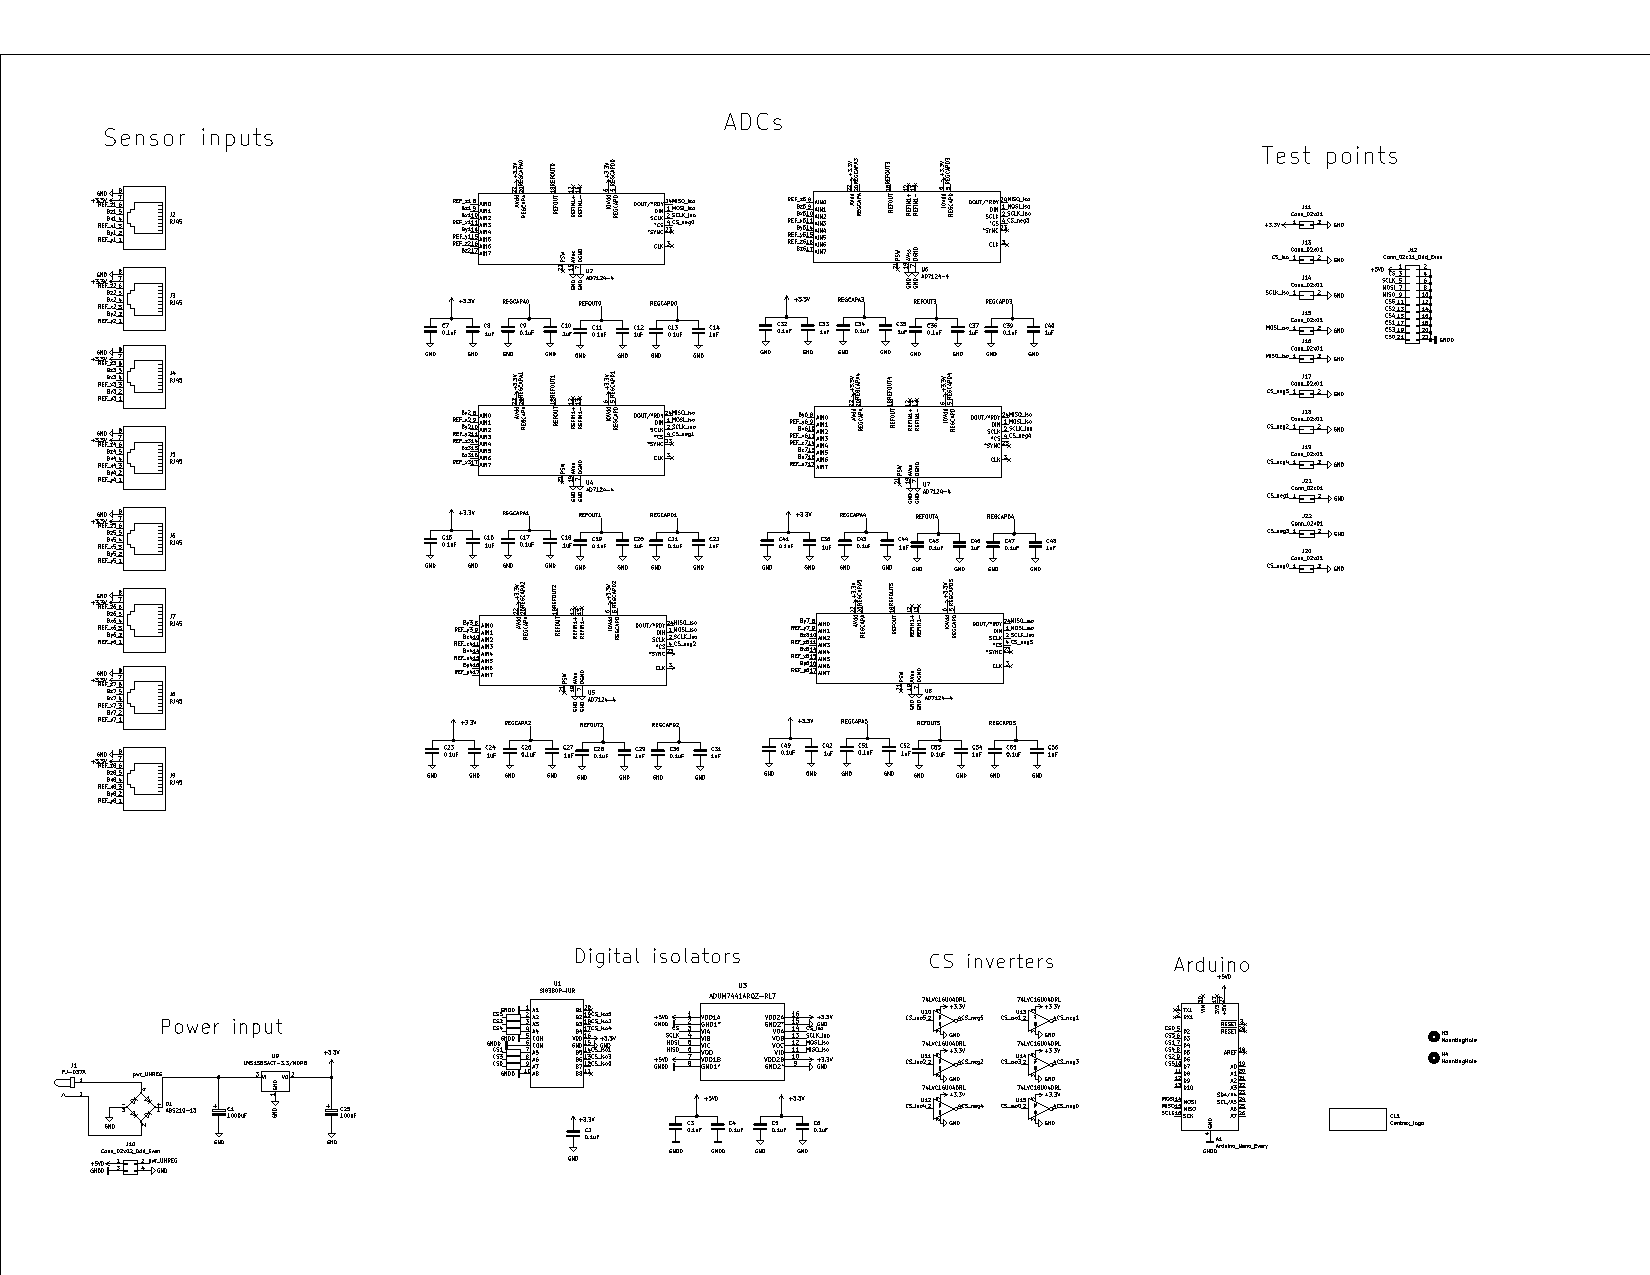
\includegraphics[width=\textwidth]{figs/schematics/multiADC.pdf}
   \caption{MultiADC v1.1 schematic}
  \label{multiadc_schem}
\end{figure}

\begin{figure}
   \centering
  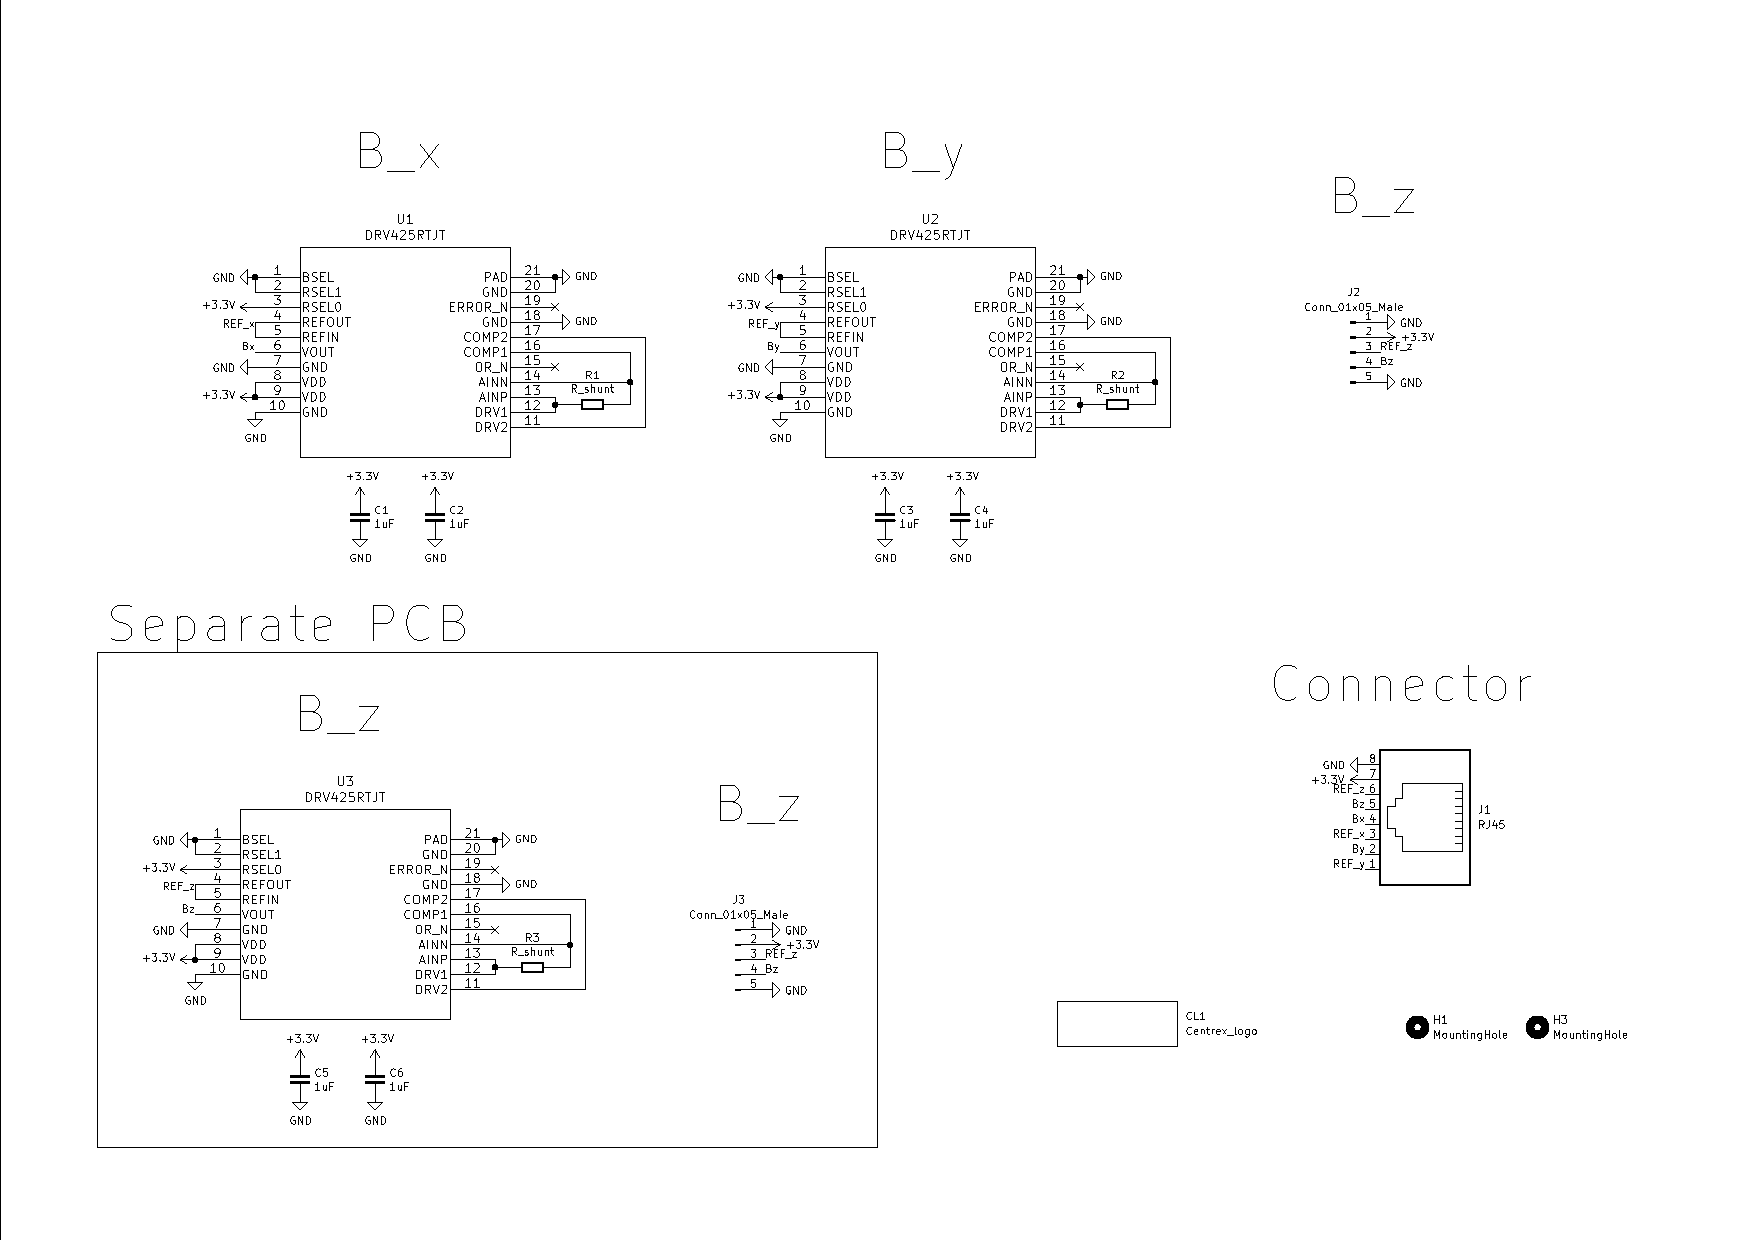
\includegraphics[width=\textwidth]{figs/schematics/magnetometer.pdf}
   \caption{Magnetometer v3.2 schematic}
  \label{magnetometer_schem}
\end{figure}

\begin{figure}
   \centering
  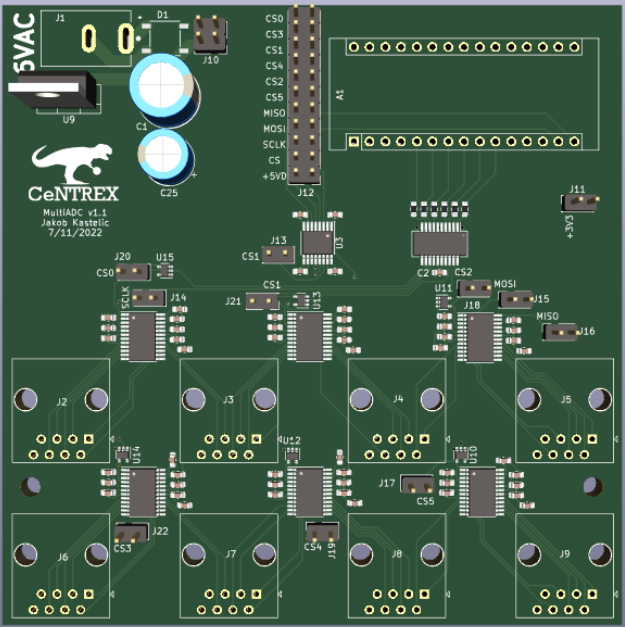
\includegraphics[width=.49\textwidth]{figs/todo/multiadc.png}
  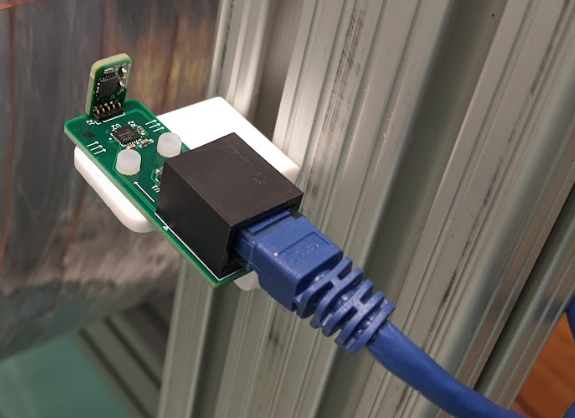
\includegraphics[width=.49\textwidth]{figs/todo/drv425.png}
   \caption[MultiADC v1.1, Magnetometer v3.2.]{\part{Left} MultiADC v1.1.
   \part{Right} Magnetometer v3.2.}
  \label{multiADC}
\end{figure}

\subsection{HV control}

\begin{figure}
   \centering
  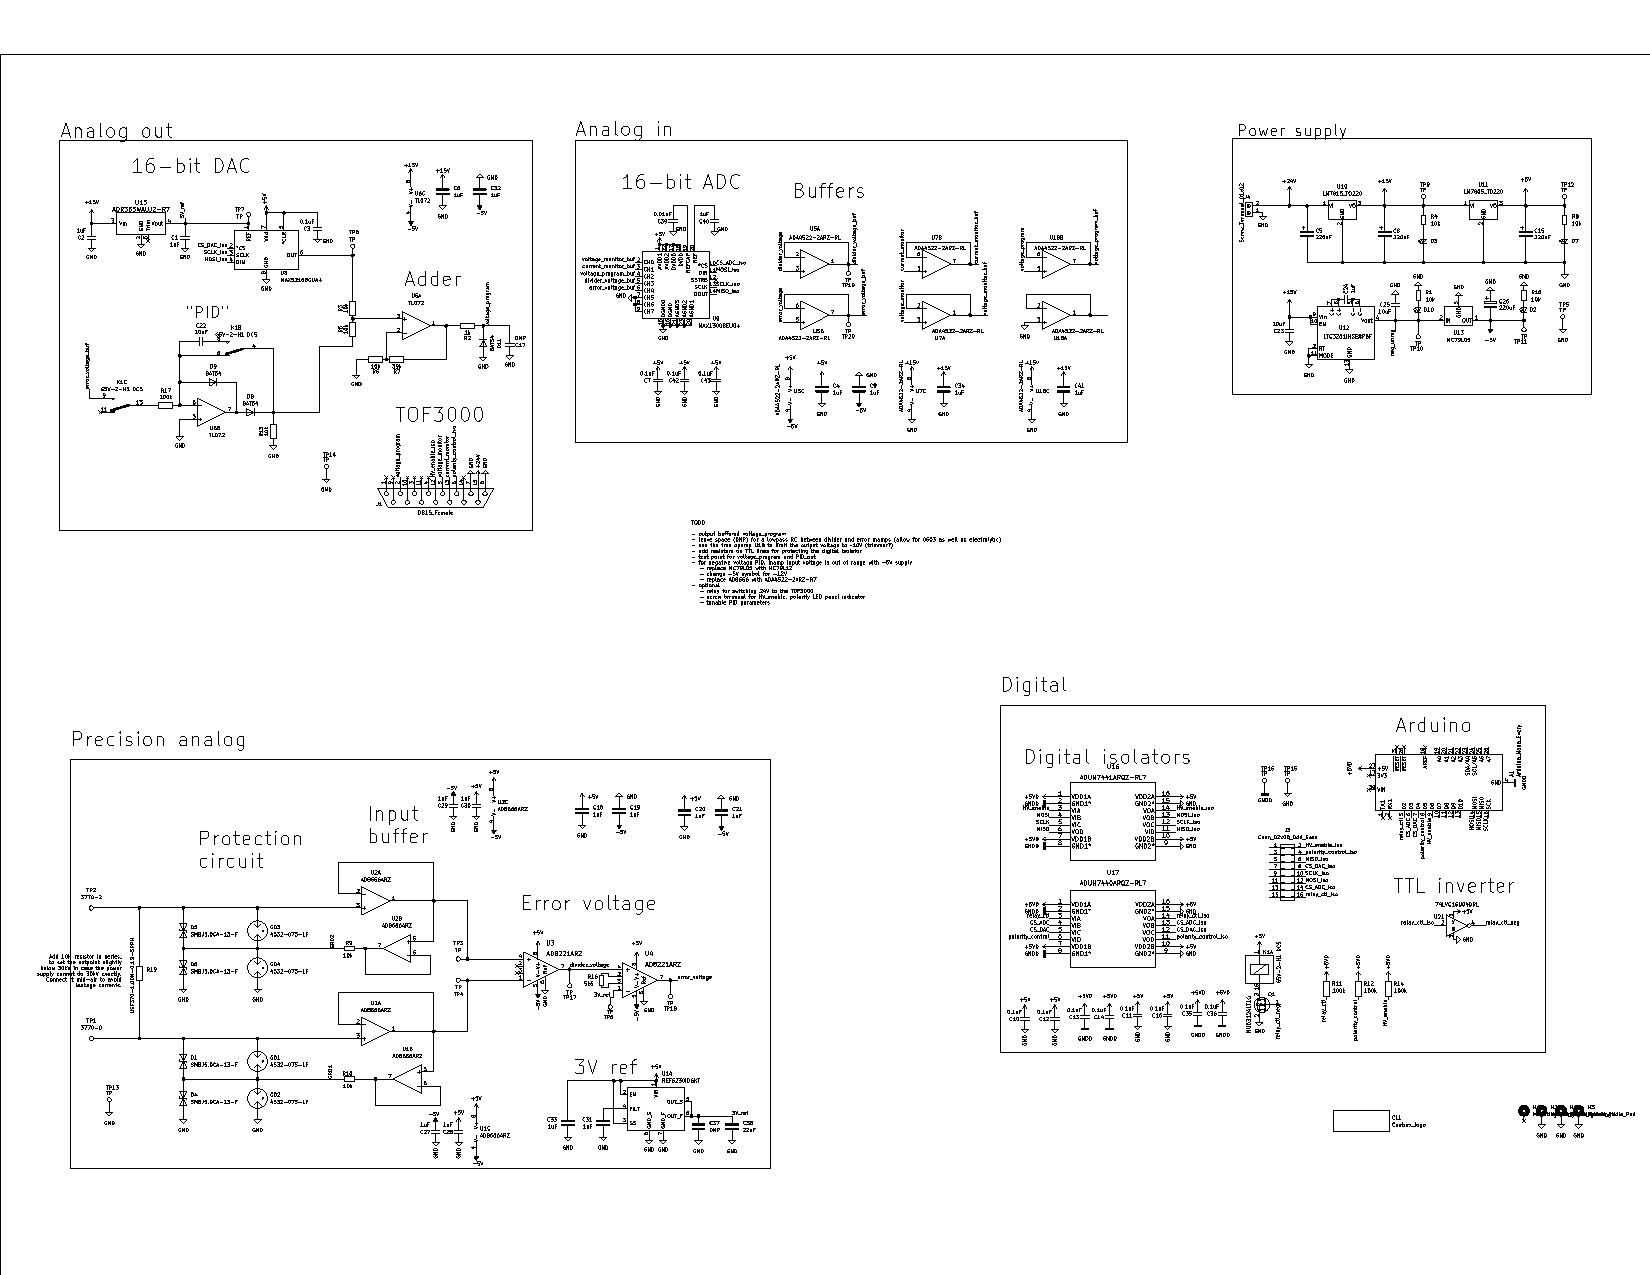
\includegraphics[width=\textwidth]{figs/schematics/HV_control.pdf}
   \caption{HV\_control v1.3 schematic}
  \label{HVctl_schem}
\end{figure}

\begin{figure}
   \centering
  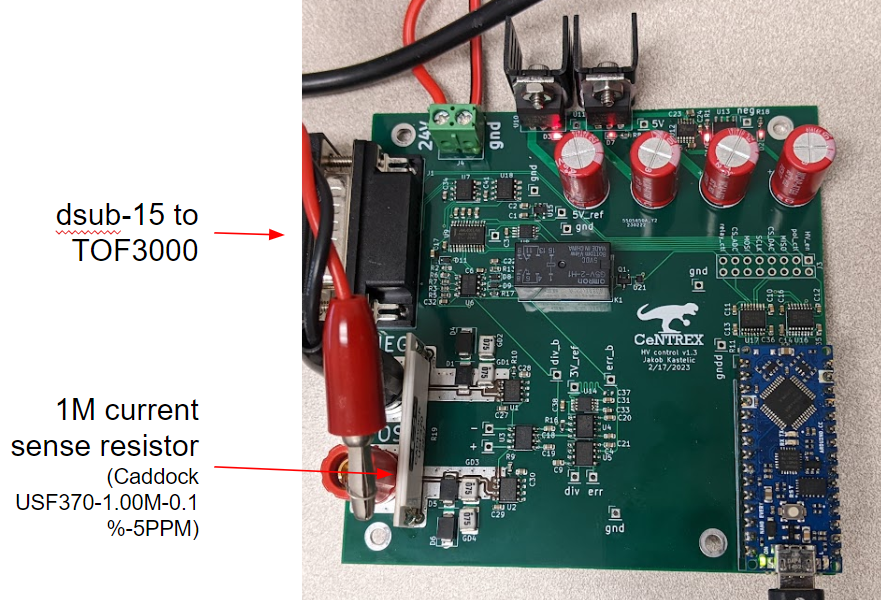
\includegraphics[width=.49\textwidth]{figs/todo/HV_ctl.png}
  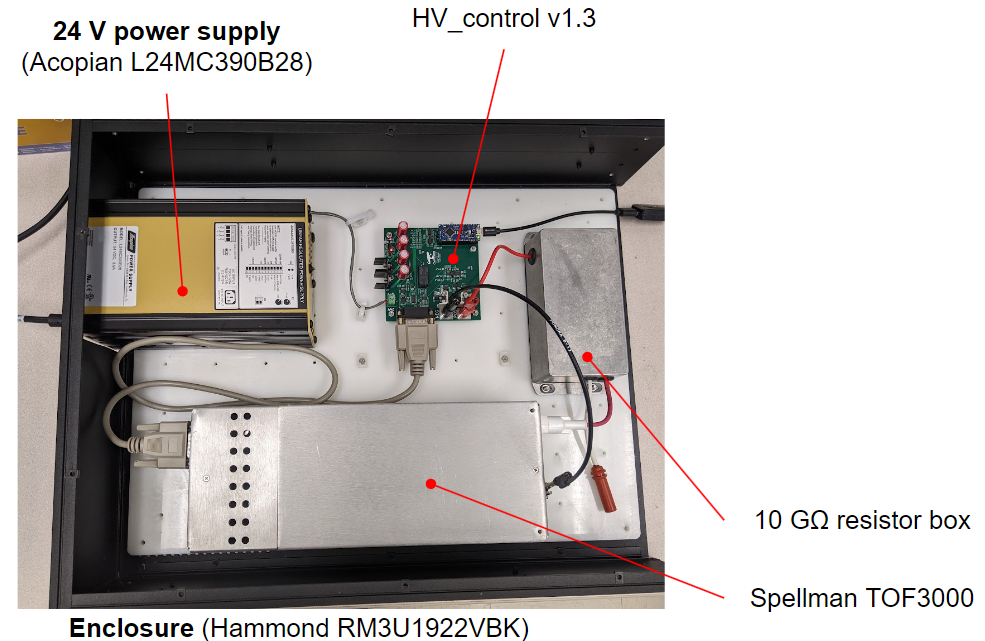
\includegraphics[width=.49\textwidth]{figs/todo/HV_rack.png}
   \caption[HV\_control v1.3, enclosure with HV electronics.]{\part{Left}
   HV\_control v1.3. \part{Right} Enclosure with HV electronics.}
  \label{multiADC}
\end{figure}
